%%%%%%%%%%%%%%%%%%%%%%%%%%%%%%%%%%%%%%%%%%%%%%%%%
%
%	MSc THESIS TEMPLATE
%	developed for my master thesis at the Universitá di Torino
%
%	by Eugenio Senes (eugenio.senes@gmail.com)
%
%	released under MIT license, so share, modify and enjoy, but quoting the author !
%
%%%%%%%%%%%%%%%%%%%%%%%%%%%%%%%%%%%%%%%%%%%%%%%%%

%% DOCUMENT CLASS (alternative to book is 'report')
% Print just right page or both sides (comment the other one)
\documentclass[12pt,a4paper,openright,oneside]{book}	%%One sided
%\documentclass[12pt,a4paper,openright,twoside]{book}	%%Double sided

\usepackage[most]{tcolorbox}


%% SET MARGINS OF THE PAGES
\usepackage{geometry}
\geometry{a4paper,portrait, left=35mm, right=20mm, top=35mm, bottom=30mm}
\usepackage[section]{placeins}
%% HEADERS AND FOOTERS
\usepackage{fancyhdr}
\pagestyle{fancy}
\fancyhf{} 			%clears default header and footer
\rhead{} 			%right head
\lhead{ \leftmark} 	%left head
\rfoot{\thepage}
%%consider using also chead, cfoot, lfoot
%coherce the plain stile to this (e.g. the first page of every chapter)
\fancypagestyle{plain}{
	\fancyhf{}
	\rfoot{\thepage}
	\renewcommand{\headrulewidth}{0pt}
	\renewcommand{\footrulewidth}{0pt}
}
%% CLEAR PAGE WITHOUT NUMBER AT THE BEGINNING OF CHAPTERS
\let\origdoublepage\cleardoublepage
\newcommand{\clearemptydoublepage}{%
  \clearpage
  {\pagestyle{empty}\origdoublepage}%
}
%% ALLOW PAGE ROTATION
\usepackage{lscape}

%% HYPERTEXT SETUP
\usepackage{hyperref}
\hypersetup{
    colorlinks,
    citecolor=black,
    filecolor=black,
    linkcolor=black,
    urlcolor=black
}
%% PDF SETTINGS
\hypersetup{
    pdfauthor={AuthorName},
    pdftitle={shortTitle},
    pdfsubject={subject},
    pdfkeywords={keyword1, keyword2}
}
%% FONTS AND SYMBOLS
\usepackage[utf8]{inputenc}
\usepackage{amsfonts}		%%fonts for the mathematical rendering of formulas
\usepackage{amssymb}
\usepackage{amsmath}
%% CHAPTERS STRUCTURE
\usepackage[italian]{babel} %%Set English as main language of the document
%% FIGURES
\usepackage{graphicx}
\usepackage{subfigure}		%%allow side by side figures with single caption
%% TABLES
\usepackage{multirow}		%%allow to merge rows in the tables
\usepackage{booktabs}		%%allow use of \toprule, \midrule, \bottomrule in tables
%%CAPTIONS
\usepackage{caption}
%% BIBLIOGRAPHY
\usepackage[babel]{csquotes}
%% CODE LISTINGS
\usepackage{listings}		%%allow to use code listings

%% HYPENATON
\hyphenation{te-si pip-po paperino}	%manual hyphenation


%%%%%%%%%%%%%%%%%%%%%%%%%%%%%%%%%%%%%%%%%%%%%%%%%
%%%% BEGIN DOCUMENT
\begin{document}

%%%%%% HEAD  OF THE DOCUMENT
\frontmatter
%%FRONT PAGE
\begin{titlepage}
%upper part
\begin{center}
{{\Large{\textsc{Universit\`a degli studi di Torino \\}}}} \vspace{5mm} {\small{\bf SCUOLA DI SCIENZE DELLA NATURA\\ \vspace{3mm}
Corso di Laurea Magistrale in Informatica}}
\vspace{5mm}
\end{center}
%logo
\begin{center}

\includegraphics[scale=.3]{head/logo.png}
\end{center}
%title
\begin{center}
\vspace{5mm}
{\LARGE{\bf Appunti del corso di Reti neurali e Deep Learning}}
%{\LARGE{\bf SECOND ROW TITLE}}
\end{center}
\hfill
\begin{minipage}[t]{0.47\textwidth}\raggedleft
\vspace{20mm}
{\large{\bf Autori:\\
Falchi Lorenzo\\
Picone Corrado (come il comico)}}
\end{minipage}
\vspace{10mm}
\begin{center}
{\large{\bf 
Anno Accademico 2024/2025}}
\end{center}

\end{titlepage}
\newpage\null\thispagestyle{empty}\newpage

%\begin{titlepage}
%upper part
\begin{center}
{{\Large{\textsc{Universit\`a degli studi di Torino \\}}}} \vspace{5mm} {\small{\bf SCUOLA DI SCIENZE DELLA NATURA\\ \vspace{3mm}
Corso di Laurea Magistrale in Fisica}}
\vspace{5mm}
\end{center}
%logo
\begin{center}

\includegraphics[scale=.3]{head/logo.png}
\end{center}
%title
\begin{center}
\vspace{5mm}
{\large{\bf Tesi di Laurea Magistrale\\}}
\vspace{5mm}
{\LARGE{\bf THE FANCY TITLE\\ OF MY FANCY THESIS\\}}
%\vspace{5mm}
%{\LARGE{\bf SECOND ROW TITLE}}
\end{center}
\vspace{20mm}
%reatori e candidato
\vspace{11mm}
\par
\noindent
\begin{minipage}[t]{0.47\textwidth}
{\large{\bf Relatore:\\
Prof. Zio Paperone}}\\
\vspace{4mm}
\\
{\large{\bf Correlatore:\\
Dr. Pico de Paperis (PAP) }}
\vspace{8mm}
{\large{\bf \\ Controrelatore:\\
Prof.ssa Nonna Papera}}
\end{minipage}
\hfill
\begin{minipage}[t]{0.47\textwidth}\raggedleft
\vspace{16mm}
{\large{\bf Candidato:\\
Paperoga}}
\end{minipage}
\vspace{9mm}
\begin{center}
{\large{\bf 
Anno Accademico 20xx/20xx}}
\end{center}

\end{titlepage}
\clearemptydoublepage
%%DEDICATION (the initial quote)
\thispagestyle{empty}
\begin{flushright}

\vspace*{30mm}

Ringrazio me stesso, ovviamente,\\
Idilio Drago (best relatore eva).\\
La mia famiglia\\
\vspace{5mm}
Agli amici:\\
Il grande BU per le lezioni di filosofia\\
Gianni per i pack opening\\
CROLE che mi ha insegnato ad usare WASD\\
Marco che mi ha insegnato ad essere Pepega\\
1298 per: elenco di cose\\
Sara per l'ansia\\
Andrea?


\end{flushright}
\newpage\null\thispagestyle{empty}\newpage

\clearemptydoublepage
%%ABSTRACT
\chapter*{Abstract}

I siti Web di phishing di oggi sono in continua evoluzione per ingannare gli utenti. La maggior parte di questi siti utilizza l’attività illegale del cybersquatting e, appropriandosi di domini che somigliano a domini commerciali famosi, ingannano l’utente spingendolo ad inserire dati personali e lucrando su di essi. Il sistema da me sviluppato utilizza una classe di modelli per l’apprendimento automatico chiamate reti neurali generative avversarie, che permette in maniera proattiva di generare domini di squatting. In particolare, utilizzo reti convoluzionali generative avversarie, per generare (partendo da un dataset di immagini) i domini che possono essere abusati. È stato poi effettuato un caso di studio reale con domini esistenti e i risultati preliminari ottenuti sono promettenti.

\clearemptydoublepage
%%INDEXES
%summary
\textit{Dichiaro di essere responsabile del contenuto dell'elaborato che
presento al fine del conseguimento del titolo, di non avere plagiato in
tutto o in parte il lavoro prodotto da altri e di aver citato le fonti
originali in modo congruente alle normative vigenti in materia di plagio
e di diritto d'autore. Sono inoltre consapevole che nel caso la mia
dichiarazione risultasse mendace, potrei incorrere nelle sanzioni
previste dalla legge e la mia ammissione alla prova finale potrebbe
essere negata.}
\tableofcontents
\clearemptydoublepage

%%%%%% BODY OF THE DOCUMENT
\mainmatter
%%INTRODUCTION
\chapter{Introduzione}
\section{Gli ingredienti del machine learning}
L'obiettivo è risolvere un problema partendo da esempi di problemi già risolti.
Per parlare di \textbf{machine learning} dobbiamo avere chiari 3 concetti fondamentali:
\begin{itemize}
    \item tasks, sono una specifica di cosa vogliamo fare (classification, regression, probability estimation;
clustering,...),
    \item model, riguardano la modalità di risoluzione del task (linear, decision trees, naive Bayes, Knn,...);
    \item features, sono il modo in cui sono descritti gli esempi da utilizzare per risolvere il problema(numerical, categorical, feature construction,
feature selection,...).
\end{itemize}

\paragraph{Esempio: l'email} 
L'obiettivo è classificare un'email come spam o come ham. Al posto di analizzare il testo, utilizziamo delle features costruite su di esso. 
Qunidi in partenza abbiamo le features, che sono raggruppate in vettori, e una etichetta che può essere spam o ham. Dobbiamo scrivere una funzione che prenda in input il vettore e restituisca l'etichetta corretta.
\textbf{SpamAssassin} è un programma per individuare email spam.
Sulla sinistra ci sono degli score che sono associati alle features; se una featutures è vera, aumenta la probabilità che l'email sia spam.

\begin{figure}
    \centering
    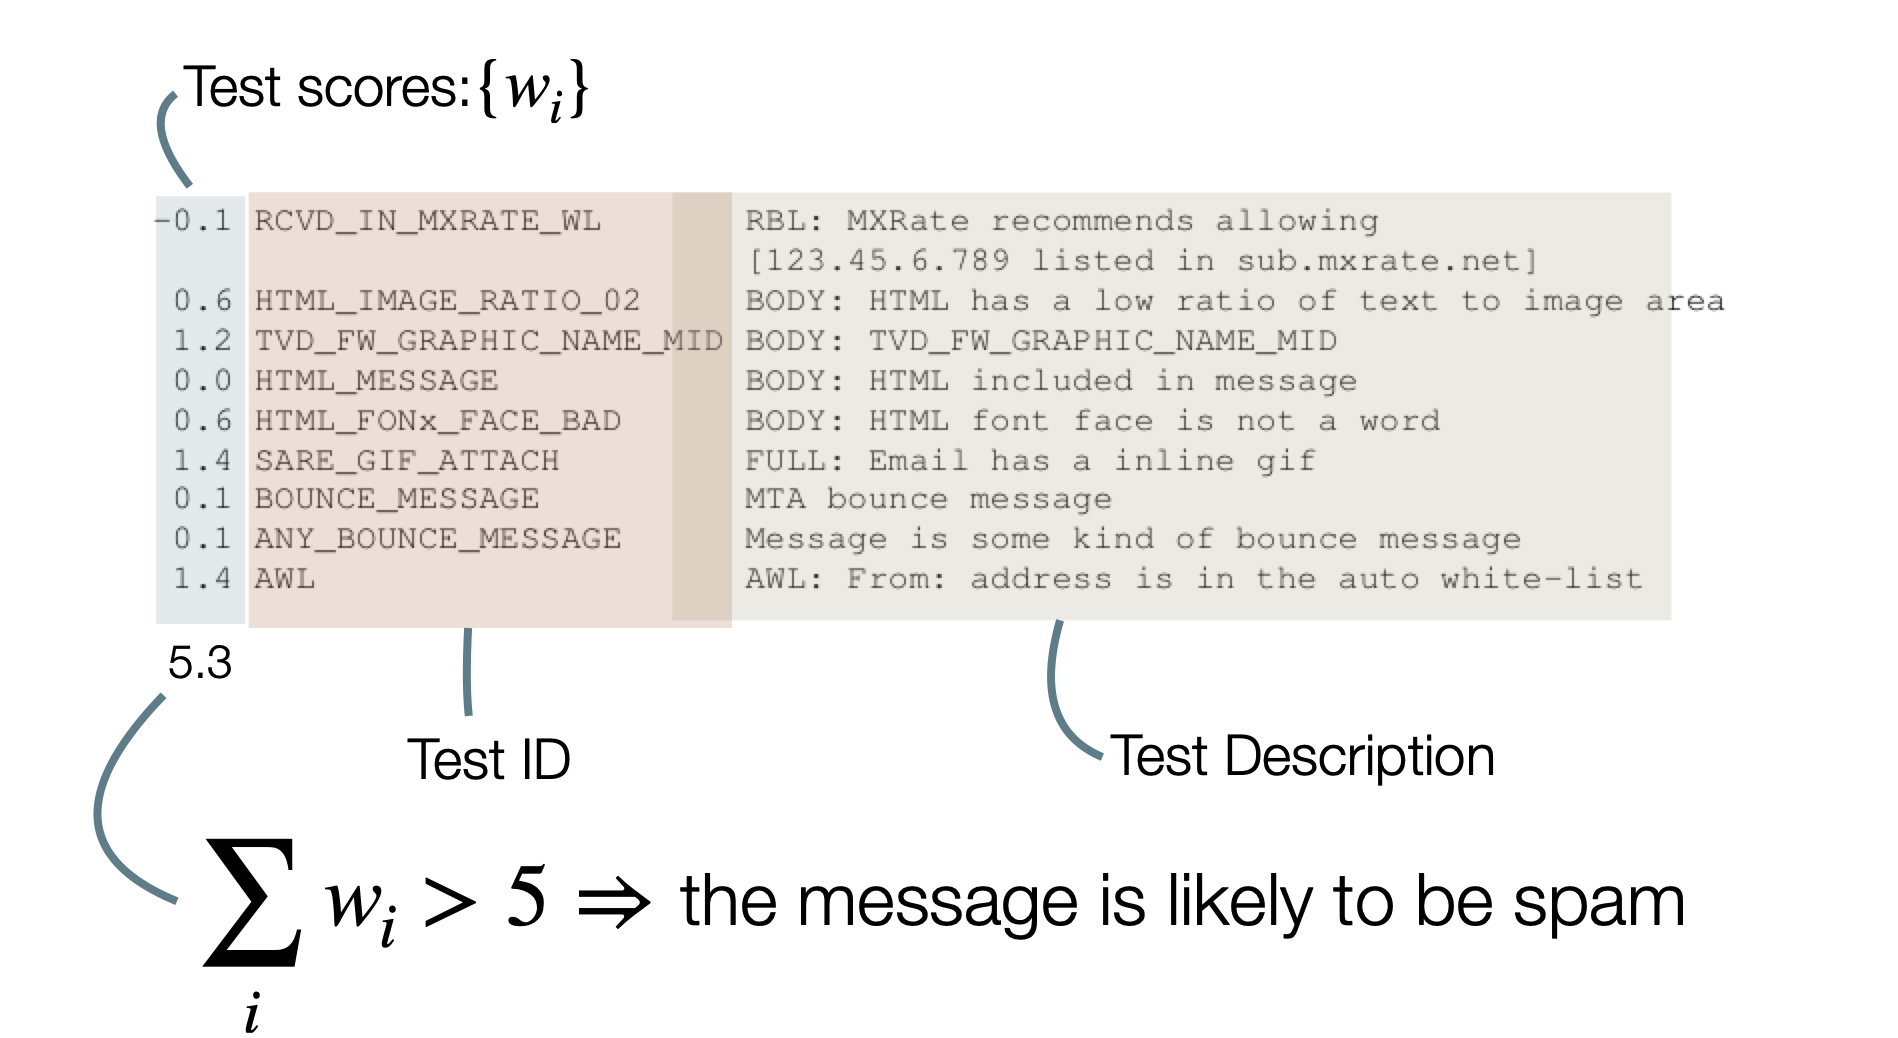
\includegraphics[scale=0.3]{images/spamAssassin.png}
    \caption{\textbf{Nota:} email \textbf{ham} è il contrario di email \textbf{spam}.}
    \label{fig:enter-label}
\end{figure}

\newpage

\paragraph{Machine Learning} \textbf{L'apprendimento automatico} è lo studio sistematico di algoritmi e sistemi che migliorano la loro \textbf{conoscenza} o \textbf{performance}(=funzione che misura quanto il modello sta facendo bene) attraverso l'\textbf{esperienza}(=esempi, features)

\begin{figure}
    \centering
    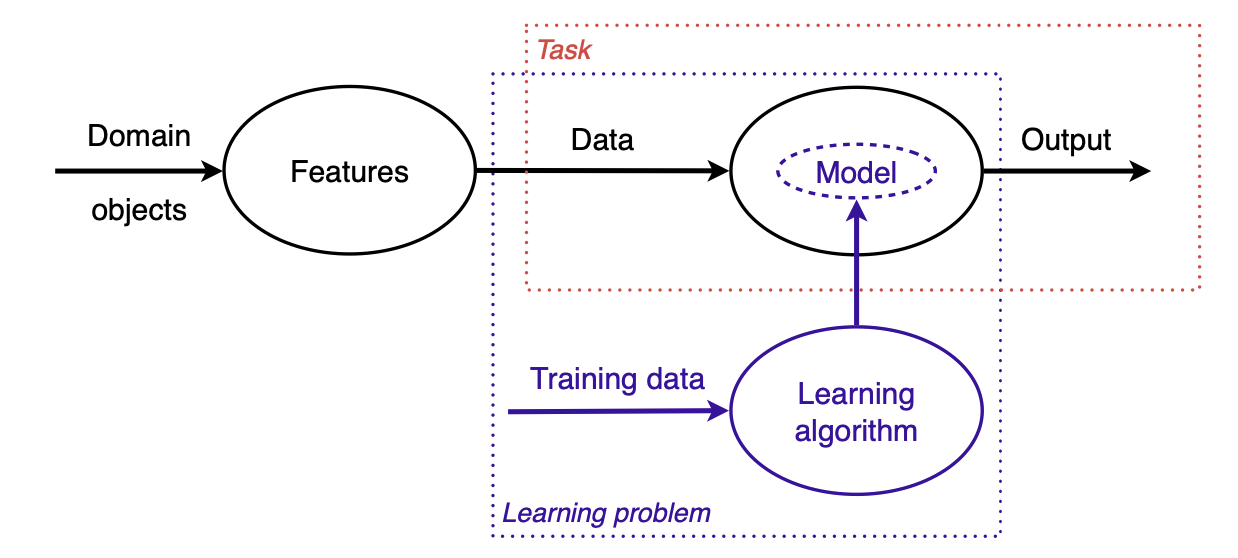
\includegraphics[scale=0.5]{images/mlModel.png}
    \caption{come il machine learning aiuta a risolvere un task}
    \label{fig:enter-label}
\end{figure}


Per risolvere un \textbf{task} devo \textbf{sfruttare un modello}, per risolvere un \textbf{problema di apprendimento} devo usare un qualche \textbf{algoritmo di apprendimento} che sviluppi un \textbf{modello} per risolverlo.

\section{Task} Ci sono sostanzialmente 2 tipi di task che si affrontano con l'apprendimento automatico: \textbf{task predittivi}  e \textbf{task descrittivi}. Nei predittivi si vuole predirre una qualche variabile a fronte delle descrizione degli esempi. I predittivi si disinguono a loro volta a seconda delle etichette che vogliamo predire:
\begin{itemize}
    \item \textbf{classificazione binaria (2 etichette) o multiclasse (più etichette)}, etichetta di tipo categorico (es. spam, ham);
    \item \textbf{regressione}, etichetta numerica;
    \item \textbf{clustering}, target nascosto.
\end{itemize}

I \textbf{task descrittivi} non hanno l'etichetta fornita, l'idea è prendere i dati forniti e fornire una descrizione di essi che sia utile a chi fa l'analisi.

\paragraph{Overfitting.} L'idea nel caso estremo è che si memorizzano troppo gli esempi e, quando si deve predirre, si tira fuori l'etichetta (se si è vista), altrimenti si va a caso. Il punto è che il modello si specializza sugli esempi forniti e non riesce a generalizzare.

\newpage
\begin{figure}
    \centering
    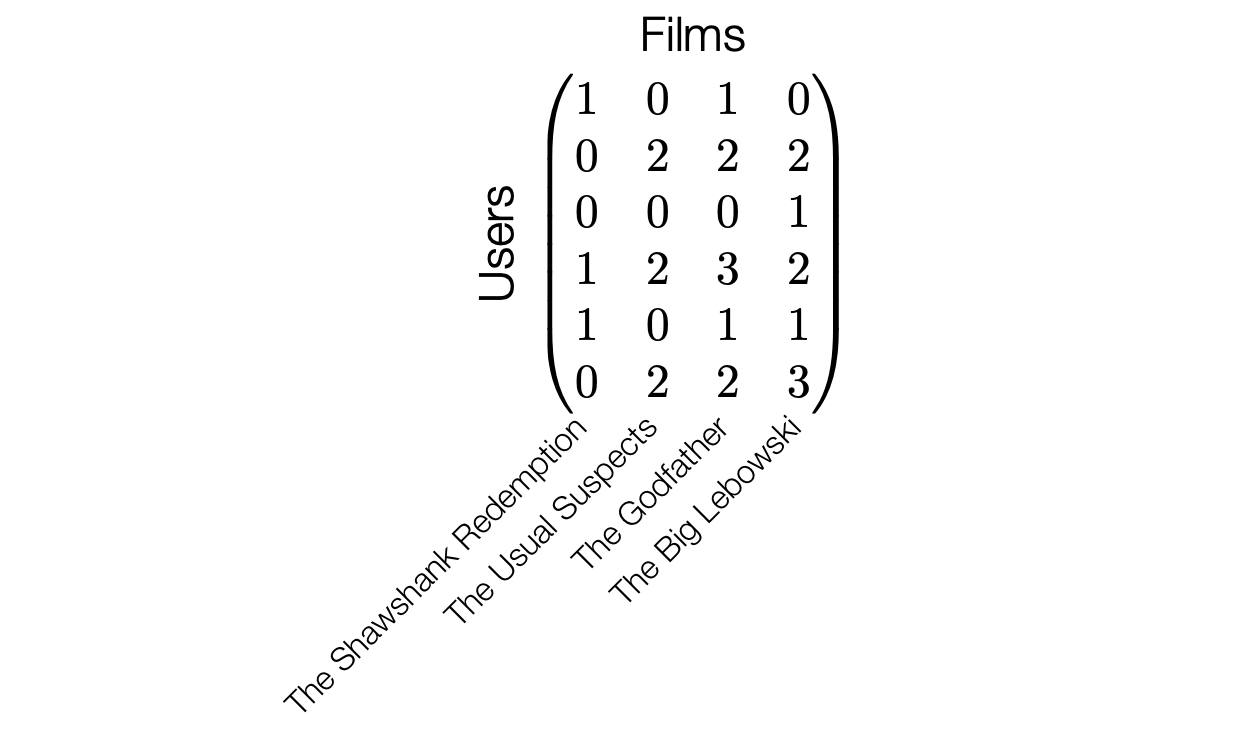
\includegraphics[scale=0.6]{images/predTask.png}
    \caption{esempio di task predittivo}
    \label{fig:enter-label}
\end{figure}

Le colonne rappresentano i film e le righe i giudizi delle persone ai quei film. Così è difficile tirare fuori qualche informazione utile, dobbiamo provare a generalizzare.

\begin{figure}[!h]
    \centering
    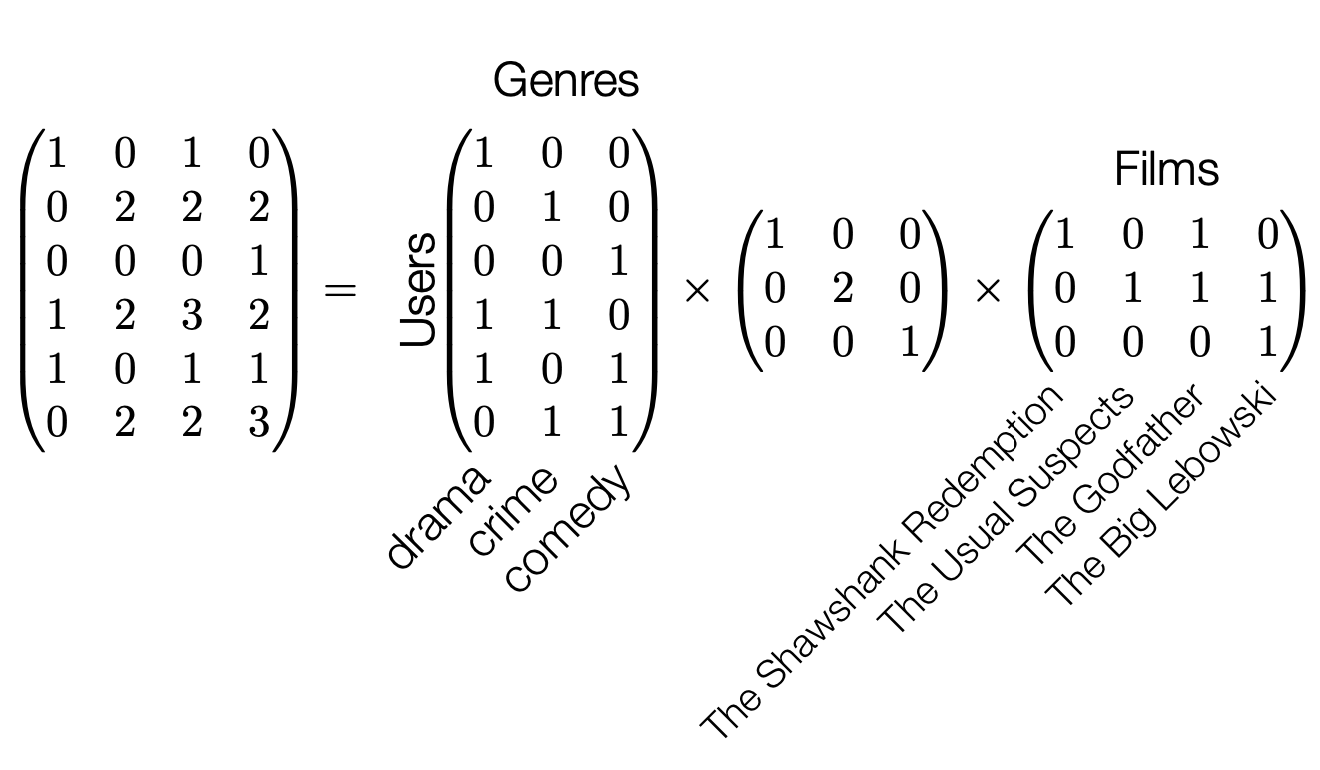
\includegraphics[scale=0.6]{images/predTask1.png}
    \caption{}
    \label{fig:enter-label}
\end{figure}

In questo modo è molto più semplice capire se ci sono relazioni tra gli utenti e i film.

\newpage

\section{Modelli} Vedremo 3 tipi di modelli:
\begin{itemize}
    \item \textbf{geometrici}, in cui si usano le intuizioni della geometria per risolvere il problema;
    \item \textbf{probabilistici}, in cui il tool principale è il calcolo della probabilità e la statistica;
    \item \textbf{logici}, in cui il tool principale sono le espressioni logiche.
\end{itemize}

In \textbf{ambito geometrico} un algoritmo di apprendimento deve \textbf{trovare l'insieme dei pesi} che permetta alla funzione di discriminare gli esempi.
\begin{equation}
    f_w(x)=w_1x_1+w_2x_2+w_3
\end{equation}
In questo esempio i pesi sono $w_1, w_2, w_3$ e gli algoritmi saranno algoritmi di ottimizzazione di qualche tipo.

\paragraph{Modelli probabilistici} Un classificatore di questo tipo, usa al posto della geometria, il calcolo della probabilità di un'etichetta avendo dei dati. Sia $X$ la descrizione del nostro esempio e $Y$ l'etichetta che vogliamo predire, quello che vorremmo fare è trovare $Y_{MAP}$ (cioè il massimo a posteriori), cioè la probabilità massima una volta che ho visto i dati.
\begin{equation}
\begin{split}
    Y_{MAP} = arg\; max_Y P(Y|X) \\
            = arg\; max_Y \frac{P(X|Y)P(Y)}{P(X)} \\
            = arg\; max_Y P(X|Y)P(Y)
\end{split}
\end{equation}
\textbf{Nota:} $P(Y|X)$ è la probabilità di avere $Y$ dato $X$.

Il denominatore non è importante perchè siamo interessati alla $Y$ che massimizza la probabilità.

Spesso $P(Y)$ non è nota quindi si usa la formula
\begin{equation}
    Y_{ML} = arg\; max_Y P(X|Y).
\end{equation}

Man mano che cresce il numero di valori da considerare, la tabella che viene fuori da questa formula è enorme (per $20$ valori sarebbero $2^{20}$ righe). In questo caso si usa uno degli algoritmi più semplici che si utilizzano con i metodi probabilistici è l'algoritmo di \textbf{Naive Bayes} che consiste nel fare un'assunzione forte su come sono fatte le probabilità (esempio assumere che $x_1$ e $x_2$ siano indipendenti tra di loro, quindi non serve calcolare l'intera tabella ma solo una per $x_1$ e una per $x_2$). 

\paragraph{Modelli logici.} Sono quei modelli in cui lo strumento che si utilizza per modellare i dati e i risultati è la \textbf{logica}. Ce ne sono molti tipi, un esempio è un classificatore logico che ha una serie di regole della forma se x allora y.
\begin{itemize}
    \item se l'email contiene la parola "viagra" stima gli odd di spam come 4:1 (spam e 4 volte più probabile rispetto ad ham);
    \item se l'email contiene la parola "blue pill" stima gli odd di spam come 3:1;
    \item altrimenti stima gli odd come 1:6.
\end{itemize}
Quindi quando si riceve un'email si applicano una dopo l'altra queste regole e la prima che matcha da la stima degli odd da cui poi si decide se dare spam o ham come etichetta corretta.

\section{Features}
Rappresentano come descriviamo i dati e hanno importanza fondamentale per arrivare ad un buon risultato. Facciamo un esempio

Supponiamo di voler approssimare $y = \cos{\pi x} $ nell'intervallo $-1 \le x \le 1$. Un'approssimazione lineare non sarebbe molto utile in questo caso, poiché il miglior adattamento sarebbe $y = 0$. Tuttavia, se suddividiamo l'asse $x$ in due intervalli, $-1 \le x < 0$ e $0 \le x \le 1$, possiamo trovare approssimazioni lineari ragionevoli in ciascun intervallo. Possiamo ottenere ciò utilizzando x sia come caratteristica di divisione che come variabile di regressione.

Un altro esempio: si vede che l'andamento è molto frastagliato.
\begin{figure}[!h]
    \centering
    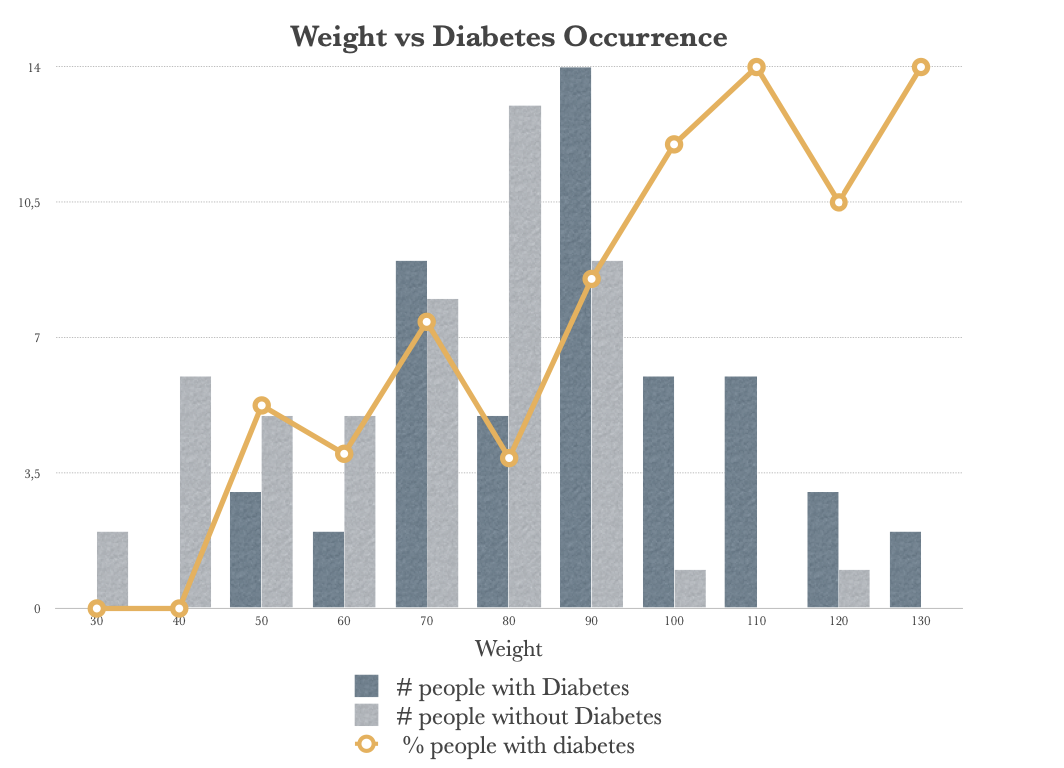
\includegraphics[scale=0.5]{images/diabetes0.png}
    \caption{Caption}
    \label{fig:enter-label}
\end{figure}

Se al posto di aggregare per 10 chili lo facciamo per 20 chili, si riesce a trattare molto meglio.
\begin{figure}[!h]
    \centering
    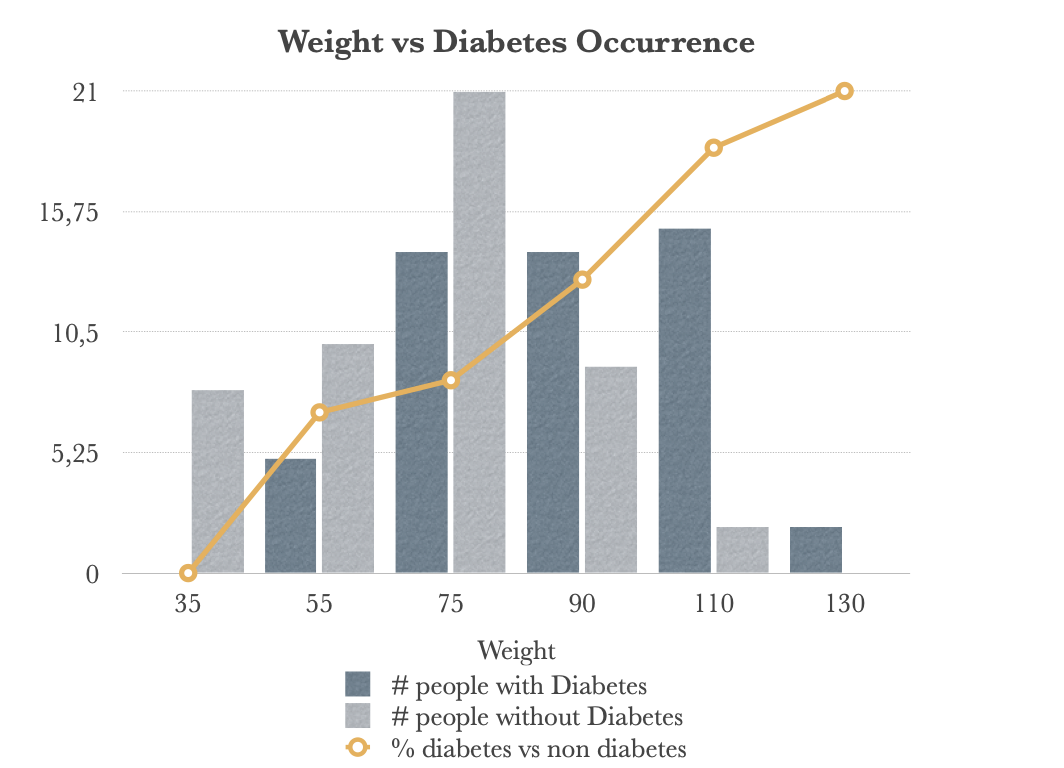
\includegraphics[scale=0.5]{images/diabetes1.png}
    \caption{Caption}
    \label{fig:enter-label}
\end{figure}

\textbf{Quindi anche solo lavorando sulle features, si riesce a semplificare di molto il problema.}
\clearemptydoublepage
% %% CHAPTERS
% add any further chapter file here
\chapter{Background}

%% SETCION1 
\section{Squatting \& phishing}
Il termine cybersquatting\cite{dewani2022handbook} si riferisce alla registrazione e all'uso non autorizzati di nomi di dominio Internet identici o simili a marchi, marchi di servizio, nomi di società o nomi personali. I registranti di cybersquatting ottengono e utilizzano il nome di dominio con l'intento in malafede di trarre profitto dalla buona volontà dell'effettivo proprietario del marchio. All'interno di questi nomi di dominio, è molto probabile incappare nel crimine comunemente chiamato Phishing. In sostanza il dominio "squattato" è il vettore che porta l'utente all'inganno, mentre il phishing è ciò che effettivamente raccoglie informazioni sensibili sugli utenti che cadono in inganno alla truffa.
Detto questo, il phishing è quindi un tipo di truffa effettuata su Internet in cui un malintenzionato cerca di ottenere informazioni riservate (dati sensibili), o peggio, dati finanziari e codici di accesso, fingendosi un ente affidabile. Tutto questo può essere sfruttato in diversi scenari applicati alla vita quotidiana di un individuo.\\
Un esempio recente è quello di utilizzare gli SMS: in un contesto in cui le persone utilizzano molto gli acquisti online, e quindi utilizzano corrieri espressi per le consegne a domicilio, è facile pensare (per un malintenzionato) di inviare un messaggio che comunica ad esempio che il proprio pacco è stato smarrito e di cliccare su un determinato link per tracciarlo. La vittima ignara della truffa clicca sul link e inserisce dati sensibili o dati bancari cadendo nella trappola del malintenzionato.\\
Questo esempio può essere applicato identico in un contesto in cui si utilizzano Mail al posto di SMS. Qui il tutto è ancora più ingannevole: oltre al testo è possibile usare come vettori dell'attacco delle immagini: il malintenzionato utilizza delle immagini che ricordano molto pagine web di cui si fida la vittima ma in cui si nascondono hyperlink che indirizzano a pagine di phishing.
\begin{figure}
  \centering
  \begin{minipage}[b]{0.4\textwidth}
    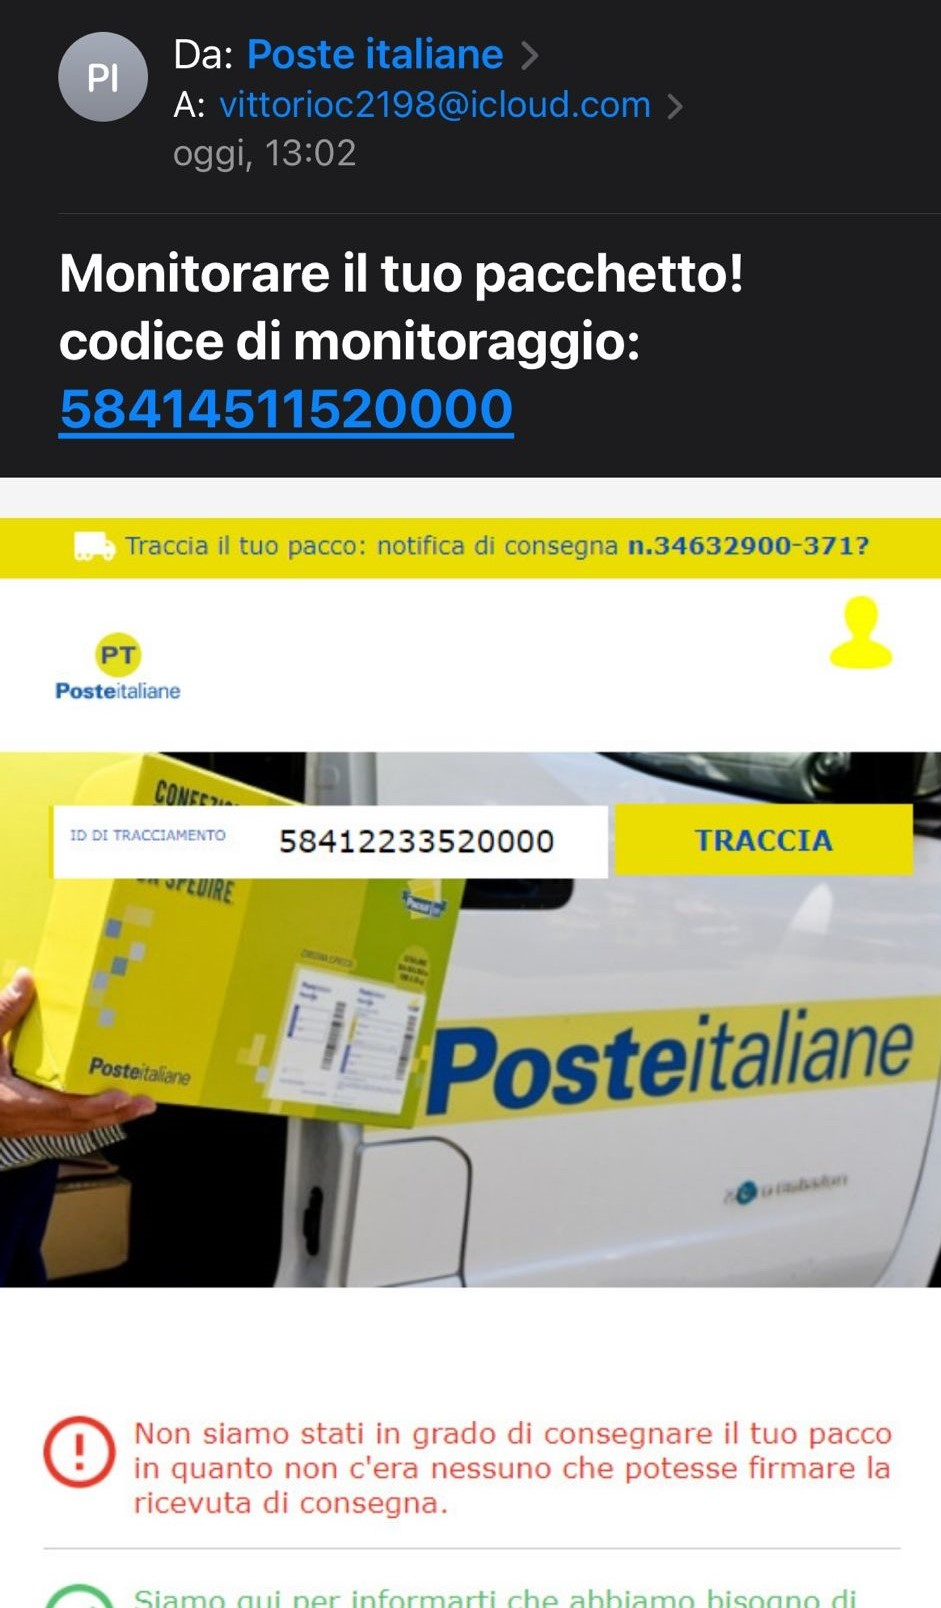
\includegraphics[width=\textwidth]{pictures/phishing1.jpeg}
    \caption{Mail Phisging}
    \label{fig:phish1}
  \end{minipage}
  \hfill
  \begin{minipage}[b]{0.4\textwidth}
    
\includegraphics[width=\textwidth]{pictures/phishing2.jpeg}
    \caption{SMS Phishing}
    \label{fig:phish2}
  \end{minipage}
\end{figure}\\
La figura \ref{fig:phish1} mostra un esempio di MAIL phishing mentre la figura \ref{fig:phish2} mostra un esempio di SMS Phishing\\


%% SECTION2
\section{Tipi di squatting}
Per effettuare il phihing, i malintenzionati utilizzano diverse tecniche di cybersquatting. Nella figura \ref{fig:phish2} ad esempio, viene sfruttato quello che viene chiamato "typo-squatting": viene acquistato un dominio che si basa su errori di battitura/digitazione. Come si può notare questo dirotta l'utente verso un sito differente da quello che voleva raggiungere.
Ovviamente le minacce non si circoscrivono solamente a typosquatting.\\
In generale vengono definiti 5 tipi di cybersquatting:
\begin{itemize}
    \item typo: come spiegato sopra, sono quei domini che si basano su errori di battitura e digitazione.
    
    \item homoglyph: questo tipo di squatting invece è uno dei più ingannevoli. Utilizza il fatto che molti caratteri tipografici sono simili tra loro. Nel dominio google, posso sostituire una 'o' con una lettera simile, ad esempio 'ŏ' (goŏgle.com).\\
    Questo tipi di dominio vengono chiamati IDN (internationalized domain name). Sono appunto nomi di dominio che contengono caratteri di alfabeto non latini (cinese, cirillico, greco, etc...). Questi nomi di dominio vengono salvati sui server DNS come stringhe ASCII utilizzando la trascrizione Punycode come visto nella Tabella~\ref{table:tab1}.
    \begin{table}[!h]
        \centering
        \caption{}
        \begin{tabular}{|l|l|}
        \hline
            IDN              & Punycode                     \\ \hline
            www.facebŏŏk.com & www.xn--facebk-tgba.com      \\
            www.googlè.com   & www.xn--googl-8ra.com        \\
        \hline
        \end{tabular}
        \label{table:tab1}
    \end{table}
    
    \item bit: questa forma di cybersquatting si basa su errori di bit-flip che si verificano durante il processo di richiesta DNS. Questi cambi di bit possono verificarsi a causa di fattori quali hardware difettoso o interferenze elettromagntiche.
    
    \item combo: il combosquatting aggiunge termini familiari negli URL che gli utenti incauti potrebbero non notare a prima vista. Questa tecnica si basa su analisi statistiche dei termini più utilizzati nelle pagine di enti affidabili, ad esempio, su instagram si usa molto la parola "story", "stories", "tags". Sapendo questo è possibile creare domini di squatting concatenando il dominio originario con uno dei termini più utilizzati: instagram-stories.com, instagram-tags.com, e così via.
    
    \item wrongTLD: Tutte le tecniche di squatting di cui sopra si
    concentrano sul nome di dominio ma ignorano il TLD. questa tecnica si riferisce a domini che cambiano il TLD ma mantengono il nome di dominio uguale. Per esempio, google.kekw appartiene alla categoria wrongTLD.
\end{itemize}
Sul web\footnote[1]{https://www.catonetworks.com/blog/cato-networks-adds-protection-from-the-perils-of-cybersquatting/} è possibile reperire dati e grafici riguardanti il numero di domini abusati, quale tipologia viene più utilizzata e quale marchio è più preso di mira dai malintenzionati del caso.
La figura \ref{fig:cakesquatting}, ad esempio mostra un grafico a torta che illustra le tipologie più utilizzate.
Ovviamente chi abusa del cybersquatting per commettere crimini come phishing, mira ad utilizzare domini squatted di marchi che statisticamente gli utenti utilizzano più frequentemente o i più indispensabili (come le banche ad esempio). In figura \ref{fig:squatdata} una vista dei marchi che vengono presi più di mira negli ultimi anni.

\begin{figure}[!h]
  \centering
  \begin{minipage}[b]{0.9\textwidth}
    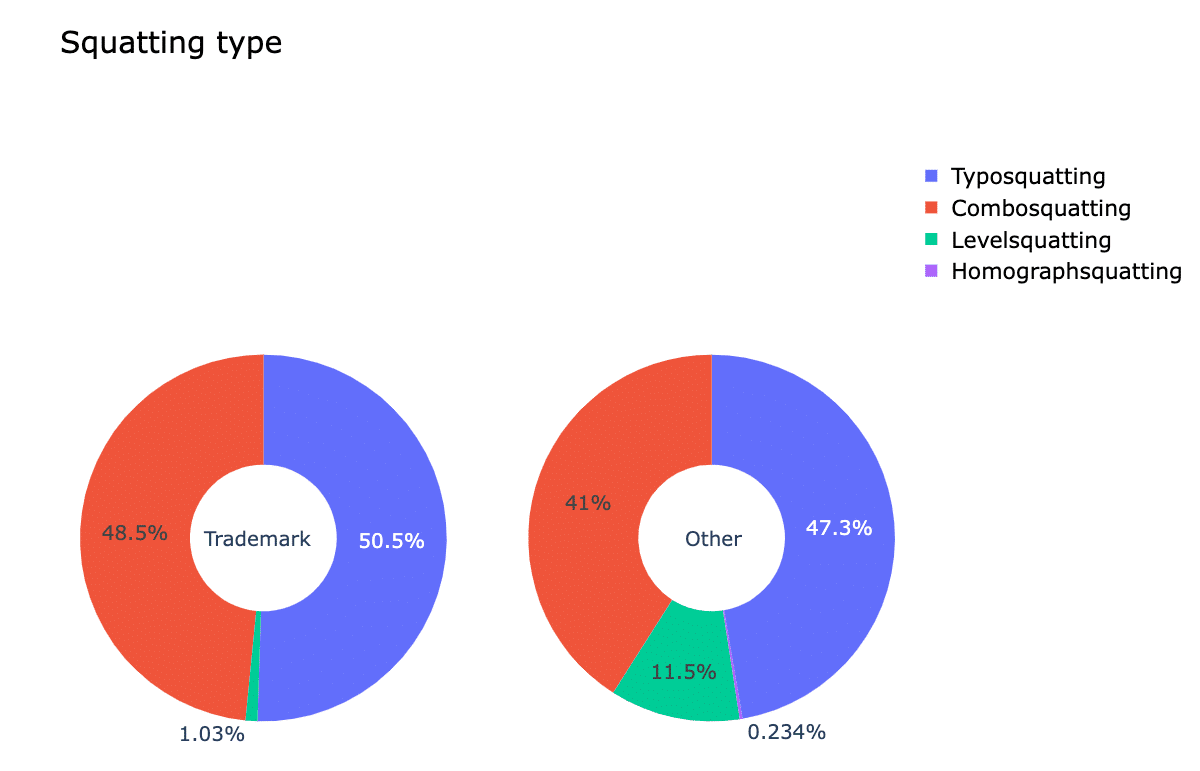
\includegraphics[width=\textwidth]{pictures/cakesquatting.png}
    \caption{Due esempi delle percentuali di squatting più utilizzate. Il primo luogo le percentuali riguardanti i marchi più famosi, in secondo luogo tutti gli altri domini}
    \label{fig:cakesquatting}
  \end{minipage}
  \hfill
\end{figure}

\begin{figure}[!h]
  \centering
  \begin{minipage}[b]{\textwidth}
    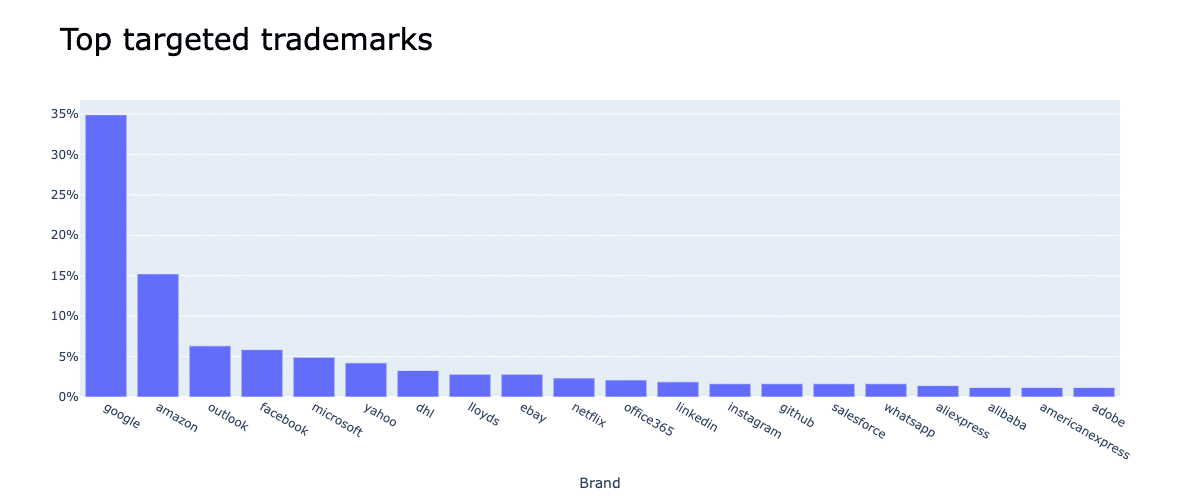
\includegraphics[width=\textwidth]{pictures/squatdata.png}
    \caption{Dati riguardanti i marchi registrati più famosi, e quali di questi vengono più presi di mira dal cybersquatting}
    \label{fig:squatdata}
  \end{minipage}
  \hfill
\end{figure}



\section{Come difendersi}
Per quanto riguarda il phishing attraverso Mail, uno dei modi migliori per difendersi è quello di analizzare il sorgente e di conseguenza analizzare i collegamenti ipertestuali per verificarne la validità. Inoltre, molti antivirus moderni, introducono un modulo per la supervisione in tempo reale delle pagine web che visitiamo: i software antivirus inglobano un modulo che confronta i domini che visitiamo con un database di URL che la compagnia ha etichettato come "malevoli"\cite{inproceedings}.\\
Un altro accorgimento che possiamo adottare è quello di analizzare la semantica e la veridicità delle informazioni[\ref{fig:mailphished}] che, ad esempio, nel caso di un SMS o di una MAIL possono essere alterate facilmente: se si riceve una Mail o un SMS in cui viene indicato che un nostro pacco è stato smarrito, ma non abbiamo ordinato nessun prodotto, è facilmente riconducibile ad un caso di phishing, senza neanche ricondurci ad analizzare il sorgente della MAIL o analizzare l'URL in oggetto.\\
Inoltre, un modo per aggirare il problema alla radice, e quindi avere la minor probabilità possibile di ricevere Mail/SMS Phishing, è proprio quello di evitare di diffondere indirizzi di posta (o numeri di telefono) ad enti/pagine web che non riteniamo del tutto affiabili. Questo perchè nel momento in cui ci iscriviamo ad un forum/applicazione/website in generale, stiamo cedendo i nostri dati alla compagnia che ne gestisce il servizio. Questi dati, nel peggiore dei casi, verranno venduti per altri scopi ad altre compagnie o chissà a chi (evitiamo di iscriverci alle newsletter).\\
In ultimo, ma non meno importante, è ciò che viene chiamato Web Crawler: Un Web crawler (spesso abbreviato in crawler) è un bot Internet che naviga sistematicamente nel World Wide Web e che è tipicamente gestito dai motori di ricerca ai fini dell'indicizzazione del Web. Il problema nasce quando non sono i motori di ricerca che utilizzano il crawling, ma enti a scopo maligno. In sostanza analizzano le pagine del WWW (scrapping) ed estrapolano qualsiasi indirizzo Mail/Numeri di telefono inserendoli successivamente in un database che utilizzeranno per i lor scopi non puliti.\\
Un'esempio più che reale è ciò che è successo a me, dopo aver pubblicato il mio indirizzo Mail sul sito di GitHub (figura \ref{fig:git}). Successivamente a quella mia azione, qualche web crawler avrà fatto scrapping della mia pagina trovando la mia Email all'interno nel sorgente dell'ipertesto (si può notare in figura \ref{fig:git2} la mail estraibile dal sorgente)
\begin{figure}
  \centering
  \begin{minipage}[b]{0.4\textwidth}
    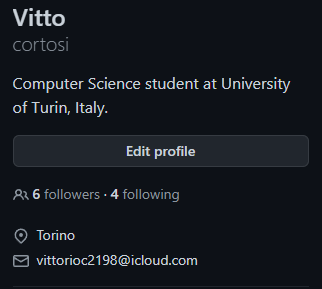
\includegraphics[width=\textwidth]{pictures/git1.png}
    \caption{La Mail inserita da me e resa pubblica sul sito GitHub}
    \label{fig:git}
  \end{minipage}
  \begin{minipage}[b]{0.56\textwidth}
    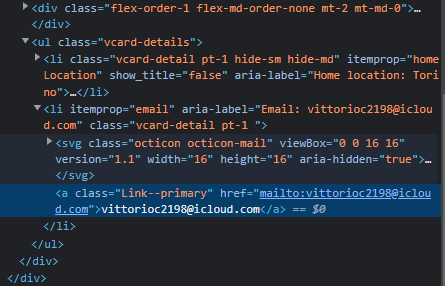
\includegraphics[width=\textwidth]{pictures/git2.png}
    \caption{La Mail che compare nel sorgente della pagina}
    \label{fig:git2}
  \end{minipage}
\end{figure}\\

\begin{figure}[!h]
  \centering
  \begin{minipage}[b]{0.5\textwidth}
    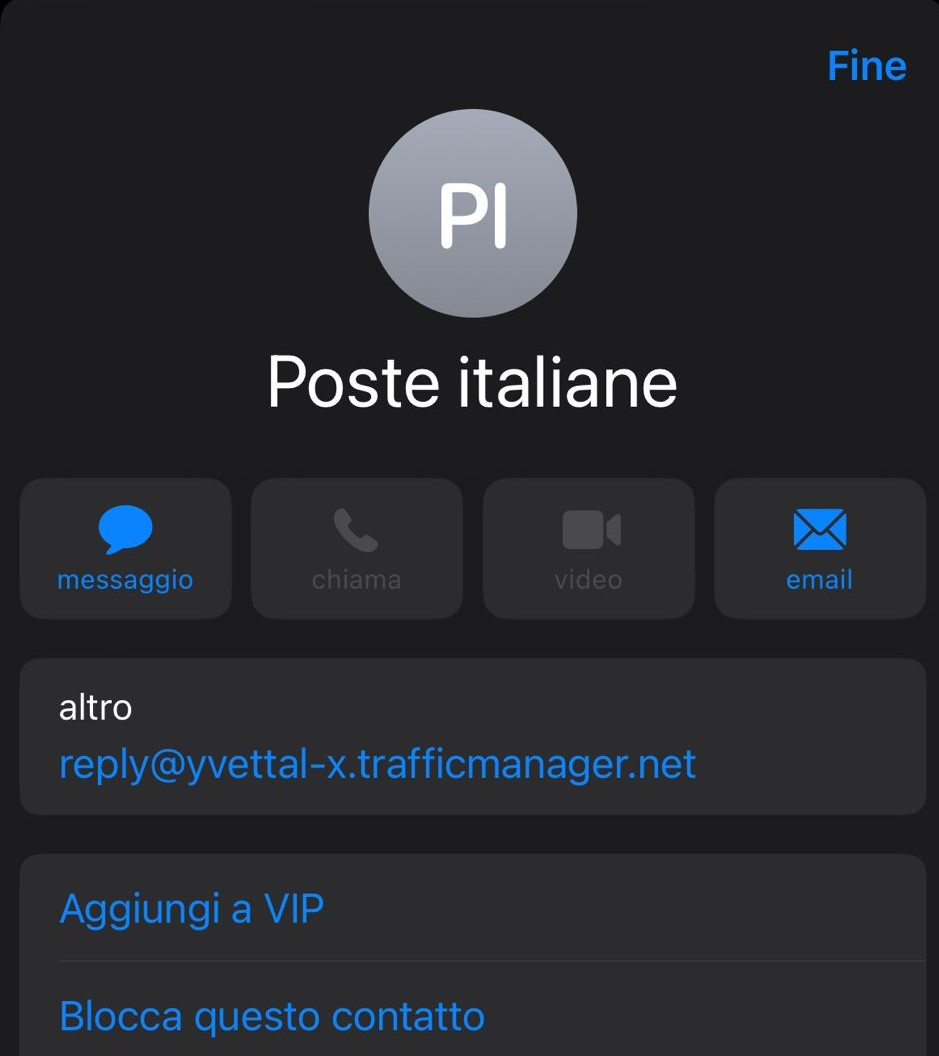
\includegraphics[width=\textwidth]{pictures/phishing3.jpg}
    \caption{In riferimanento alla figura \ref{fig:phish1}, ci si potrebbe difendere andando a controllare l'indirizzo da cui è stata inviata la mail}
    \label{fig:mailphished}
  \end{minipage}
  \hfill
\end{figure}

%% SECTION3
\section{Reti neurali generative}
Costruire un sistema in grado di generare in modo proattivo una quantità considerevole di domini di squatting non è banale. Esistono già sistemi in grado di farlo (DNSTwist è un esempio), ma come indicato dagli autori dall'articolo Needle in a Haystack\cite{10.1145/3278532.3278569}, questi generatori di domini di squatting sono in parte affidabili in quanto sono limitati in quanto non riescono a gestire in modo efficace domini di squatting combinati (combo) o domini che cambiano il TLD, inoltre, gli strumenti esistenti sono molto incompleti nel rilevamento dei domini omografici. Troviamo che strumenti come DNSTwist non riescono a mappare l'elenco completo di caratteri Unicode simili. Ad esempio, ci sono 23 diversi caratteri Unicode che sembrano simili alla lettera "un", ma DNSTwist ne cattura solo 13. Queste limitazioni danneggeranno seriamente le nostre possibilità di catturare pagine di phishing occupate.\\
Uno dei modi per cui si può pensare di generare in modo proattivo dei domini di squatting, è con l'utilizzo di Reti neurali, in particolare, utilizzando reti neurali generative.\\
Le reti neurali generative sono una classe di metodi per l'apprendimento automatico in cui due reti neurali si sfidano diventando uno l'avversario dell'altro (infatti vengono anche chiamate reti neurali generative avversarie). In questo processo, una rete neurale chiamata Generatore genera dati candidati che poi la controparte, chiamata Discriminatore, le valuta. Il generatore quindi cerca di ingannare il discriminatore generando il più possibile dati che rispecchiano quelli reali. Nella figura \ref{fig:gan1} uno schema semplice di GAN\\
\begin{figure}[!h]
  \centering
  \begin{minipage}[b]{\textwidth}
    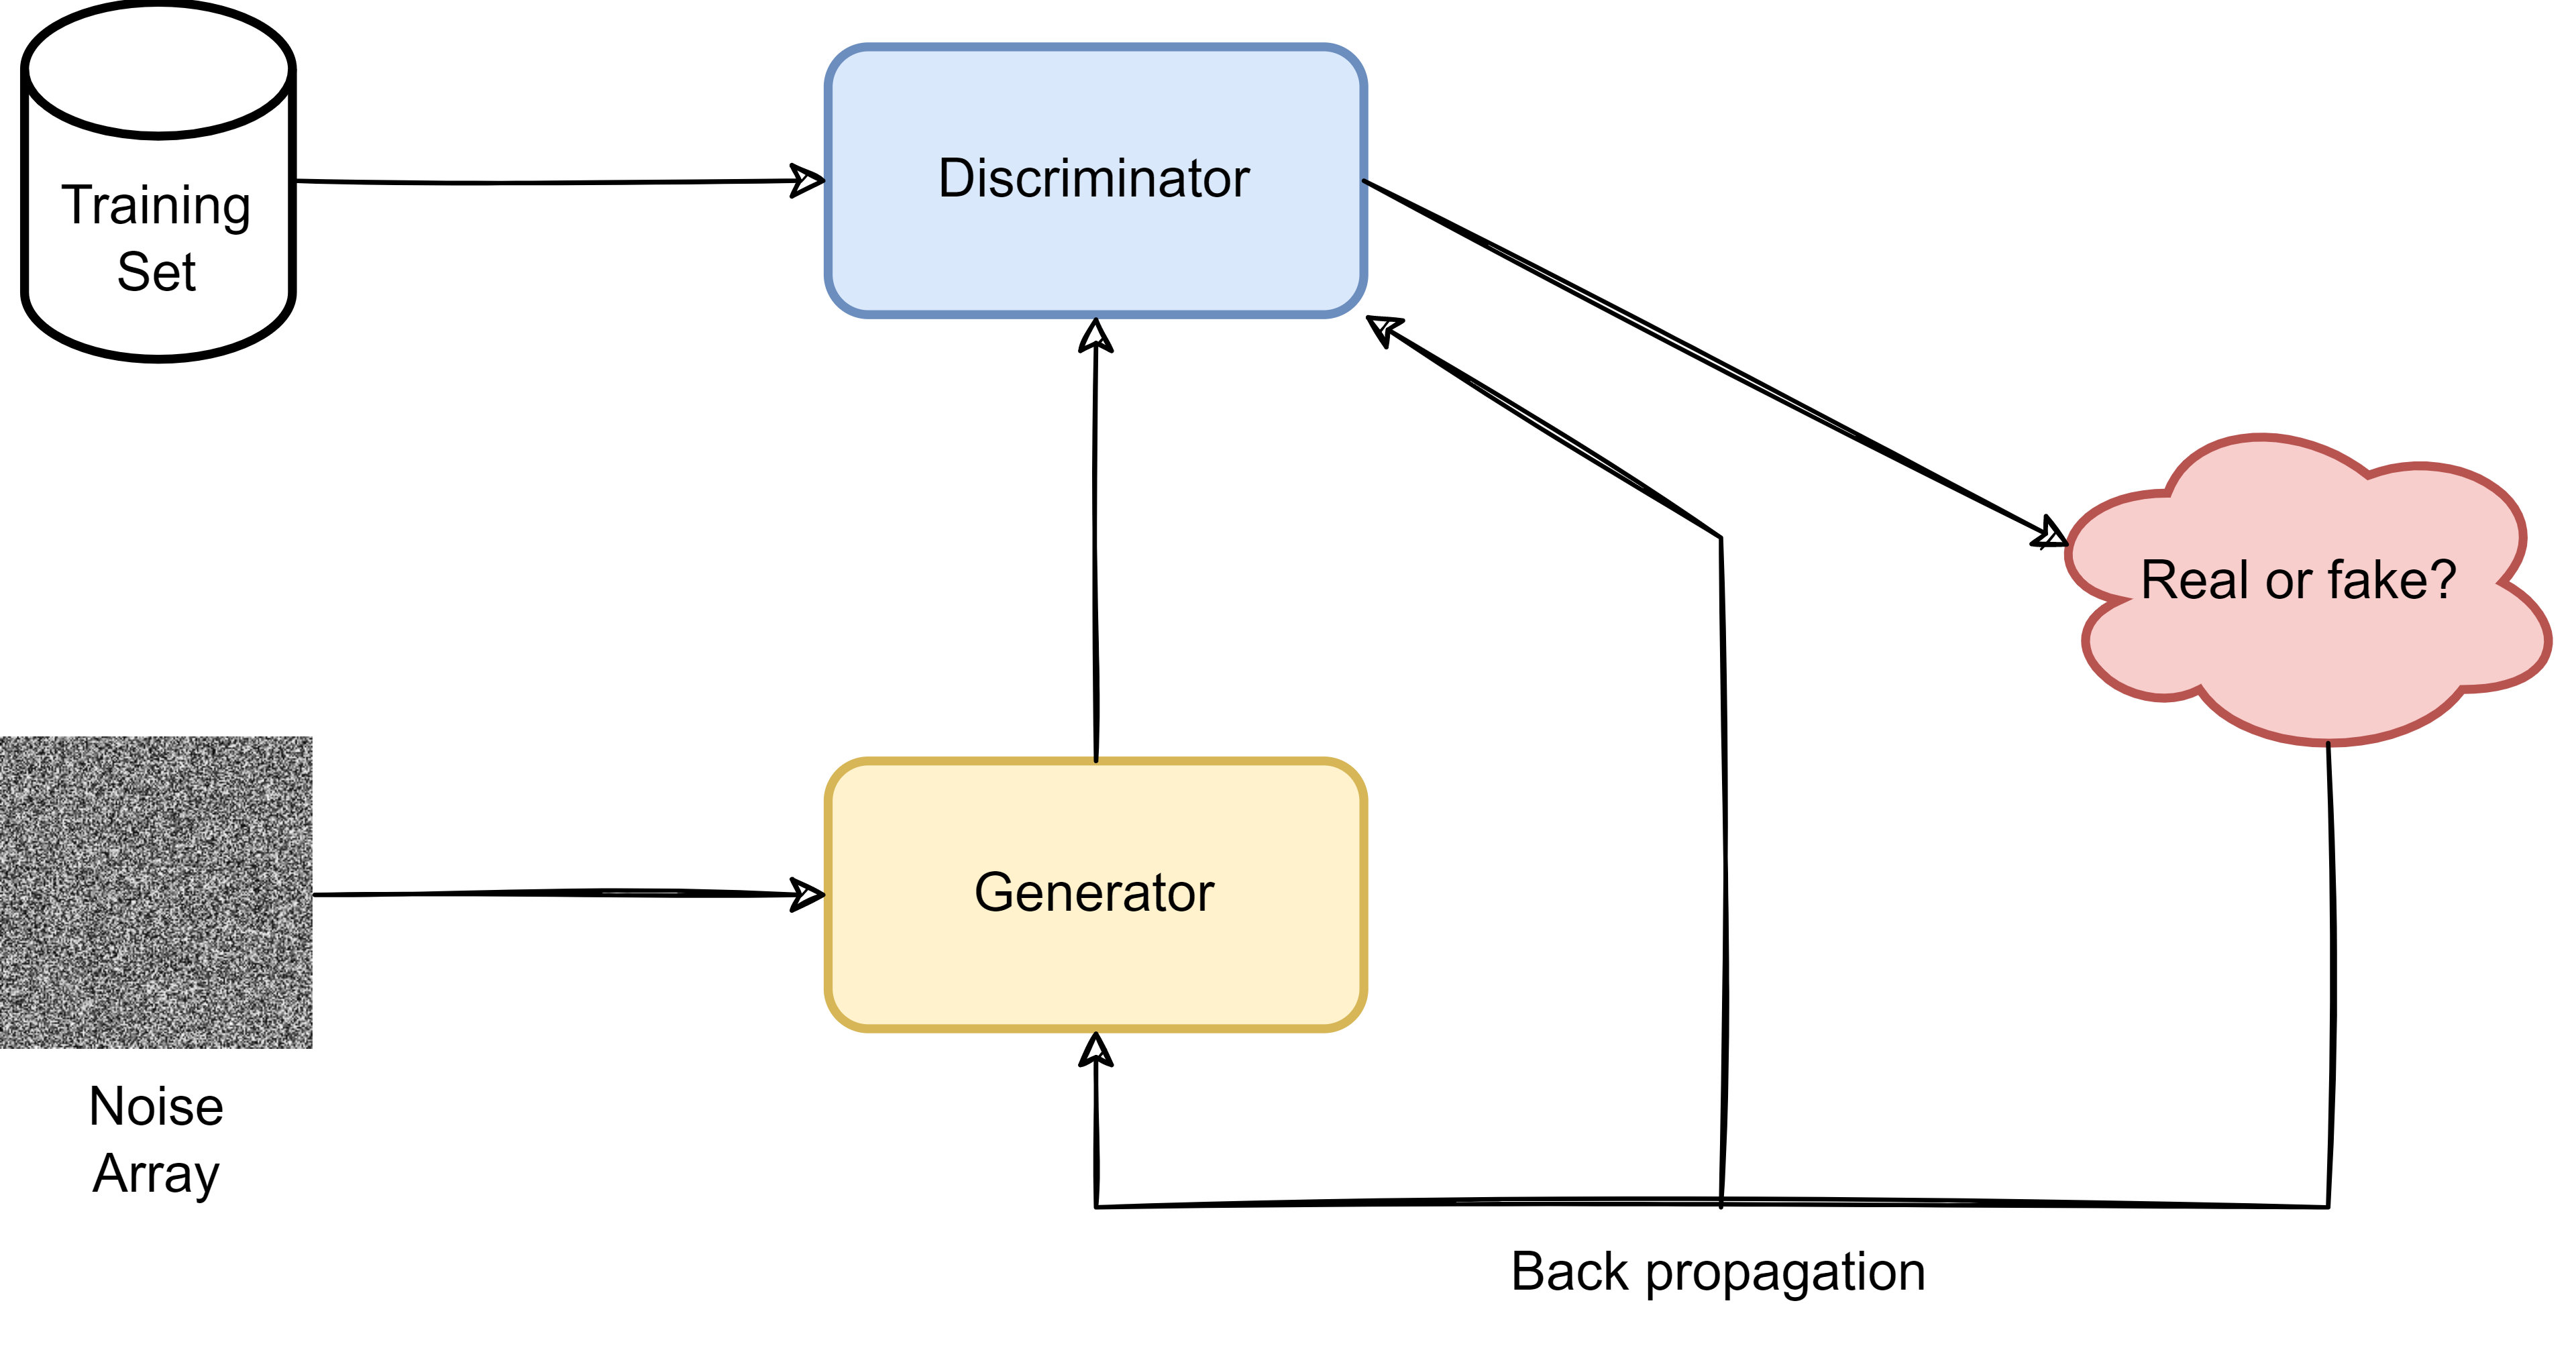
\includegraphics[width=\textwidth]{pictures/gan.png}
    \caption{Simple Gan Scheme}
    \label{fig:gan1}
  \end{minipage}
  \hfill
\end{figure}
Il modello di rete neurale generativa che utilizzerò per la generazione proattiva di domini di squatting, è chiamata Deep Convolutional Generative Adversarial Network

\section{Le DCGAN}
Le reti convoluzionali generative, seguono la filosofia delle reti generative classiche ma procedono utilizzando una struttura dei layer totalmente differente. Nelle reti generative convoluzionali, sia il generatore che il discriminatore utilizzano reti profonde costituite interamente da strati di convoluzione-deconvoluzione, ovvero da qui il nome "rete convoluzionale generativa".\\
Le reti convoluzionali (non per forza generative, CNN) sono utilizzate nell'apprendimento automatico in maniera importante soprattutto per il riconoscimento di immagini.

%% SECTION4
\section{Le GANs nella cybersecurity}
Le applicazioni\cite{9298135} per questi modelli di rete neurale sono davvero molteplici ed il potenziale è davvero enorme, in quanto, questi modelli di reti neurali possono essere istruiti a creare informazioni estremamente simili a qualsiasi dominio della vita reale: immagini, musica, audio, testo.\\
Vengono, inoltre, utilizzati anche nella branca della sicurezza informatica, la cosa meno entusiasmante è che vengono usate in primo luogo come metodo di attacco.\\
In primo luogo vengono utilizzate per eludere sistemi di riconoscimento di Malware: un sistema che genera malware appoggiandosi ad un modello di rete GAN è in grado di generare dei malware che sono non identificabili (o difficilmente) dal sistema su cui dovrà essere eseguito.\\
In secondo luogo possono essere usate per violare sistemi di autenticazione biometrica: sistemi che potrebbero basare i loro permessi di accesso attraverso l'uso della voce o del volto.
Come ultimo esempio, ma non meno importante, è l'applicazione delle GAN nei sistemi di password guessing: l'autenticazione della password è uno dei metodi più comunemente utilizzati dagli utenti che tendono a scegliere password facili da indovinare poichè utilizzano stringhe comuni. Questi tipi di stringhe sono soggetti ad attacchi chiamati password guessing in cui un utente malintenzionato tenta di accedere utilizzando un database di stringhe comuni, dizionari di parole e database di password leaked. L'efficacia dell'attacco si basa sulla capacità di testare rapidamente un gran numero di password altamente probabili rispetto a ciascun hash di password. Una tecnica avanzata si basa sull'intuizione su come gli utenti scelgono le password definendo un'euristica per le trasformazioni delle password, che include combinazioni di più parole e lettere maiuscole e minuscole, etc... Poichè lo sviluppo e il test di nuove regole ed euristiche è un'attività dispendiosa in termini di tempo e che richiede competenze specializzate, entrano in gioco le GANs. Poiché la password è una stringa codificata in testo, è possibile utilizzare un approccio basato su GAN in cui una rete neurale viene addestrata per determinare autonomamente le caratteristiche e le strutture delle password e per sfruttare questa conoscenza per generare nuovi campioni che seguono la stessa distribuzione. Le reti neurali profonde sono sufficientemente espressive da acquisire una gamma di proprietà e strutture che descrivono la maggior parte delle password scelte dall'utente e possono essere addestrate senza alcuna conoscenza o ipotesi pregressa. Ciò implica un'ampia gamma di conoscenze per indovinare le password che includono e superano ciò che viene catturato nelle regole generate dall'uomo e nei processi di generazione delle password.
\clearemptydoublepage
\chapter{Scoring and Ranking}
\section{Scoring Classifier}
Cambiamo ora tipo di classificatore: prima ne usavamo uno binario a cui davamo un esempio e restituiva 0 o 1, ora invece prendiamo un classificatore che prende un esempio X restituisce un vettore:
\begin{equation}
    \hat{s}: X \rightarrow \mathbb{R}^k
\end{equation}
con il vettore fatto così:
\begin{equation}
    \hat{s}=(\hat{s_1}(x),\dots,\hat{s_k}(x)).
\end{equation}
Più uno score è alto, più la classe associata a quello score, è considerata affidabile.
Se ci sono solo 2 classi, gli score negativi saranno dedicati alla classe $c_1$ e quelli positivi alla classe $c_2$.

Il training set continua ad essere un esempio con una classe associata, l'output è cambiato poichè restituisce, appunto, uno score.

\paragraph{Scoring Tree}
In questi alberi, alle foglie è associato uno score invece di una classe. Per calcolare gli score si fa il logaritmo del rapporto tra, in questo caso, spam e ham.
\begin{figure}[!h]
    \centering
    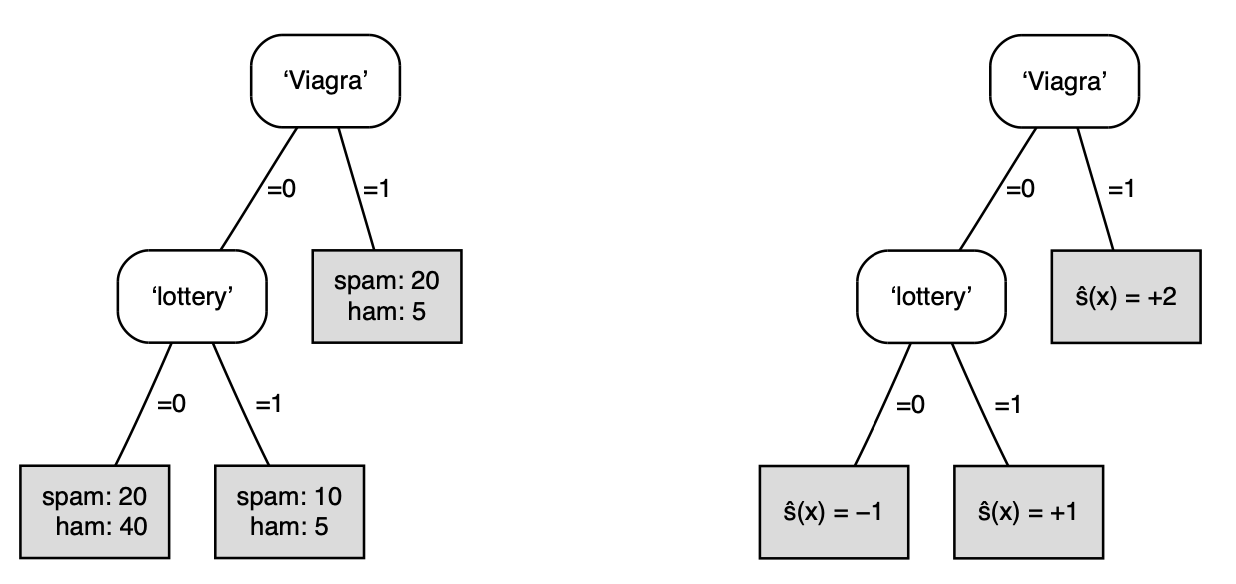
\includegraphics[scale=0.7]{images/scoringTree.png}
    \label{fig:enter-label}
\end{figure}

\paragraph{Margini.} Un \textbf{margine} è la combinazione degli score con la vera etichetta associata al modello.
\begin{equation}
    z(x)=c(x)\hat{s}(x)=\begin{cases}
        +\left|\hat{s}(x) \right| \; \text{se }\hat{s}\text{ è corretto} \\ 
        -\left|\hat{s}(x) \right| \; \text{altrimenti}
\end{cases}
\end{equation}
$c(x)$ è la classe vera che c'è nel dataset, $\hat{s}(x)$ è lo score assegnato. Per semplicità consideriamo comunque la classificazione binaria; l'idea è che il margine sia positivo quando la classificazione è corretta e negativo quando non lo è.

\paragraph{Loss function.} Una \textbf{loss function} è una funzione che misura quanto male sta facendo il modello. Spesso i problemi di apprendimento si definiscono in funzione delle loss function, come \textbf{problemi di minimizzazione della funzione}.

La funzione è definita come $L: \mathbb{R} \rightarrow [0,\infty)$ che mappa il margine $z(x)$ di un esempio ad un certo valore di loss $L(z(x))$.

Assumiamo che nel caso in cui il margine sia zero assumeremo che la loss sia $L(0)=1$. Quindi la loss sarà $L(z) \ge 1$ se $z<0$ e $0\le L(z)<1$ se $z>0$.

\begin{figure}[!h]
    \centering
    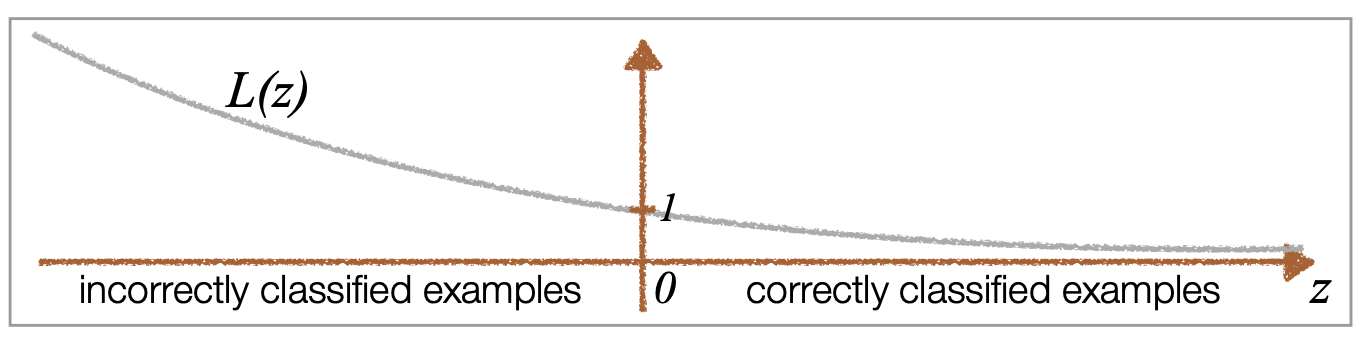
\includegraphics[scale=0.7]{images/lossFun.png}
    \label{fig:enter-label}
\end{figure}

Ci sono diversi tipi di loss function:
\begin{itemize}
    \item \textbf{0-1 loss}, la più semplice, indica che la loss è 1 se stiamo sbagliando a classificare l'esempio, 0 altrimenti
        \begin{equation}
        \begin{split}
            L_{01}(z)=1 \; \text{if} \; z\le 0 \\
            L_{01}(z)=0 \; \text{if} \; z> 0 
        \end{split}
        \end{equation}
        sommando la loss di tutti gli esempi, vediamo gli esempi che stiamo classificando male. 

        Notiamo che la funzione è discontinua
        \begin{figure}[!h]
            \centering
            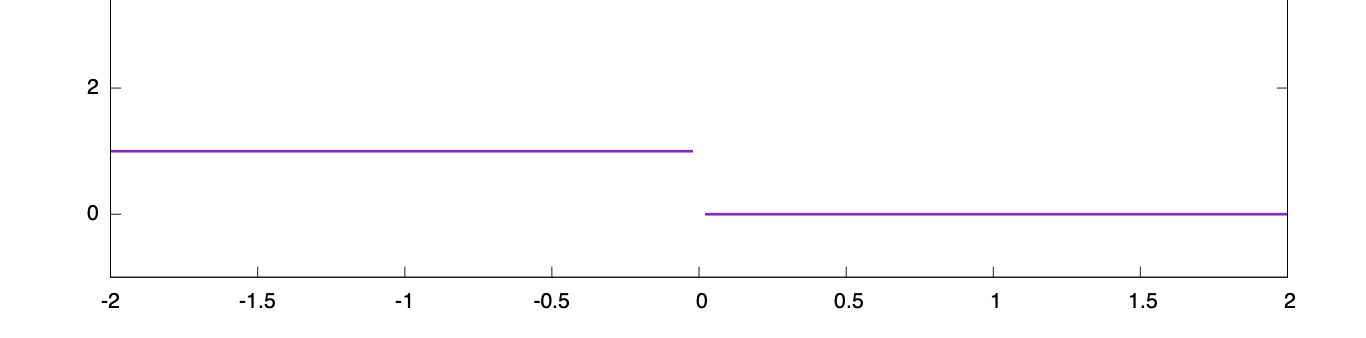
\includegraphics[scale=0.5]{images/01loss.png}
            \label{fig:enter-label}
        \end{figure}
        e la sua derivata è 0 sia a sinistra che a destra, il che vuol dire che se riesco a classificare correttamente gli esempi, non ho nessun altra informazione da utilizzare per migliorare ulteriormente il modello.
    \item \textbf{Hinge loss}, risolve parzialmente il problema della derivata,  
    \begin{equation}
        \begin{split}
            L_{h}(z)=(1-z) \; \text{if} \; z\le 1 \\
            L_{h}(z)=0 \; \text{if}\;  z> 1 
        \end{split}
    \end{equation}
    
    \begin{figure}[!h]
        \centering
        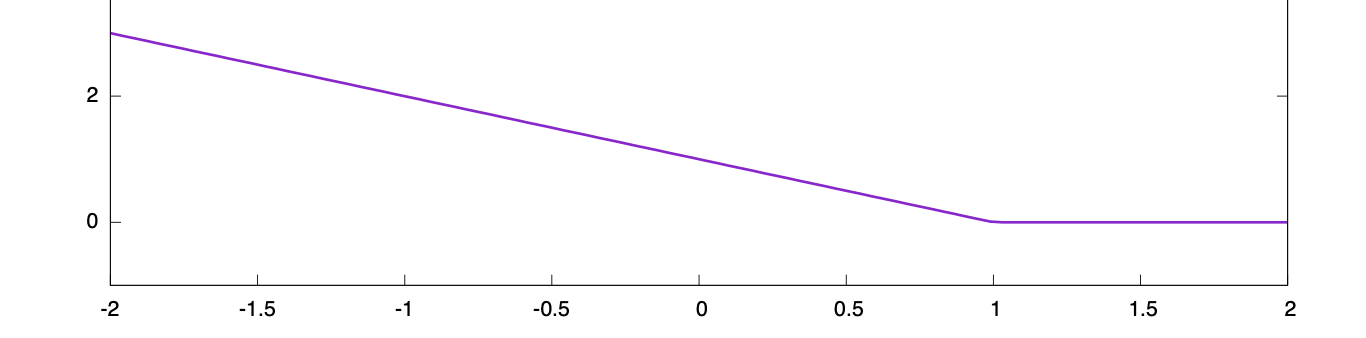
\includegraphics[scale=0.5]{images/hingeLoss.png}
        \label{fig:enter-label}
    \end{figure}
    ci permette di migliorare la classificazione anche quando siamo tra 0 e 1;
    \newpage
    \item \textbf{logistic loss}, 
    \begin{equation}
        L_{log}(z)= \log_2(1+(\exp(-z)))
    \end{equation}
    
    \begin{figure}[!h]
        \centering
        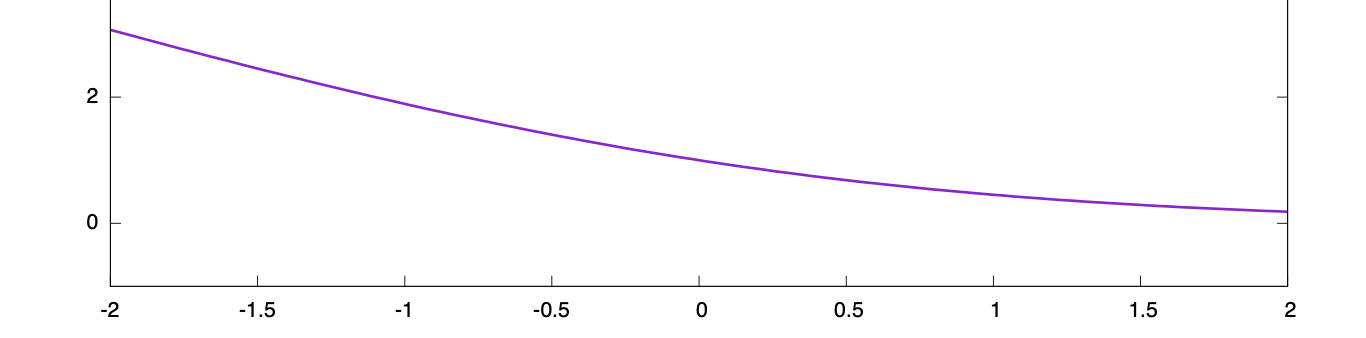
\includegraphics[scale=0.5]{images/logLoss.png}
        \label{fig:enter-label}
    \end{figure}
    è un'approssimazione della precedente, completamente continua;
    
    \item \textbf{exponential loss}, 
    \begin{equation}
        L_{exp}(z)=\exp(-z)
    \end{equation}
    
    \begin{figure}[!h]
        \centering
        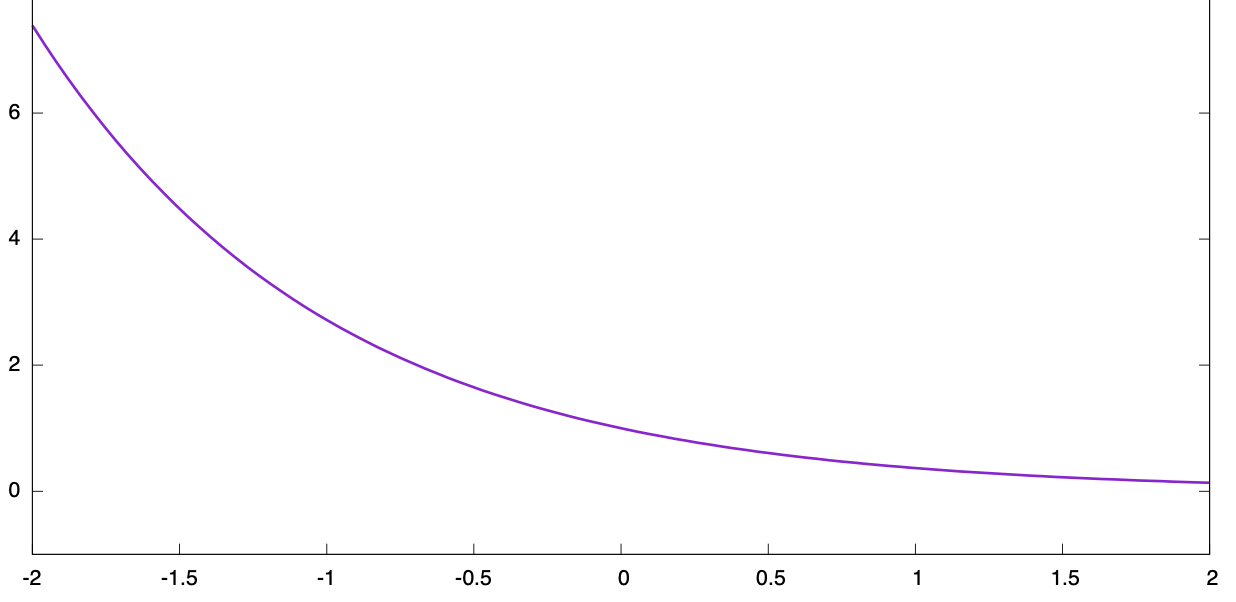
\includegraphics[scale=0.3]{images/expLoss.png}
        \label{fig:enter-label}
    \end{figure}
    \item \textbf{squared loss}, 
    \begin{equation}
        L_{sq}(z)=(1-z)^2
    \end{equation}
    
    \begin{figure}[!h]
        \centering
        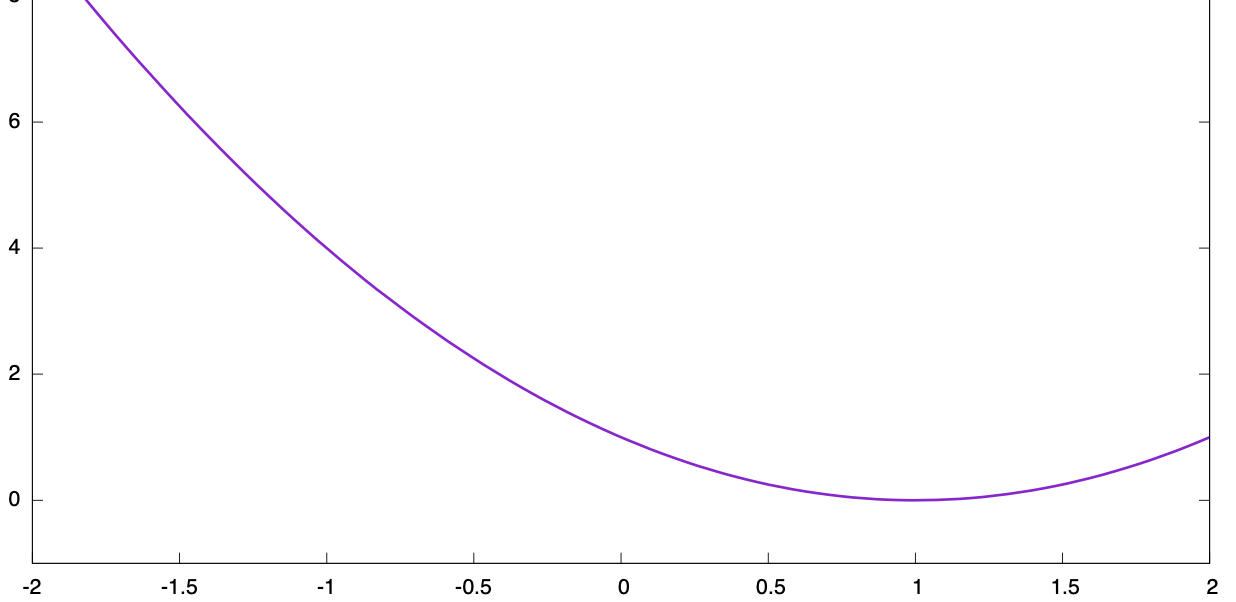
\includegraphics[scale=0.3]{images/sqLoss.png}
        \label{fig:enter-label}
    \end{figure}
\end{itemize}
Viste tutte in un unico grafico risultano l'una l'approssimazione dell'altra:
\begin{figure}[!h]
    \centering
    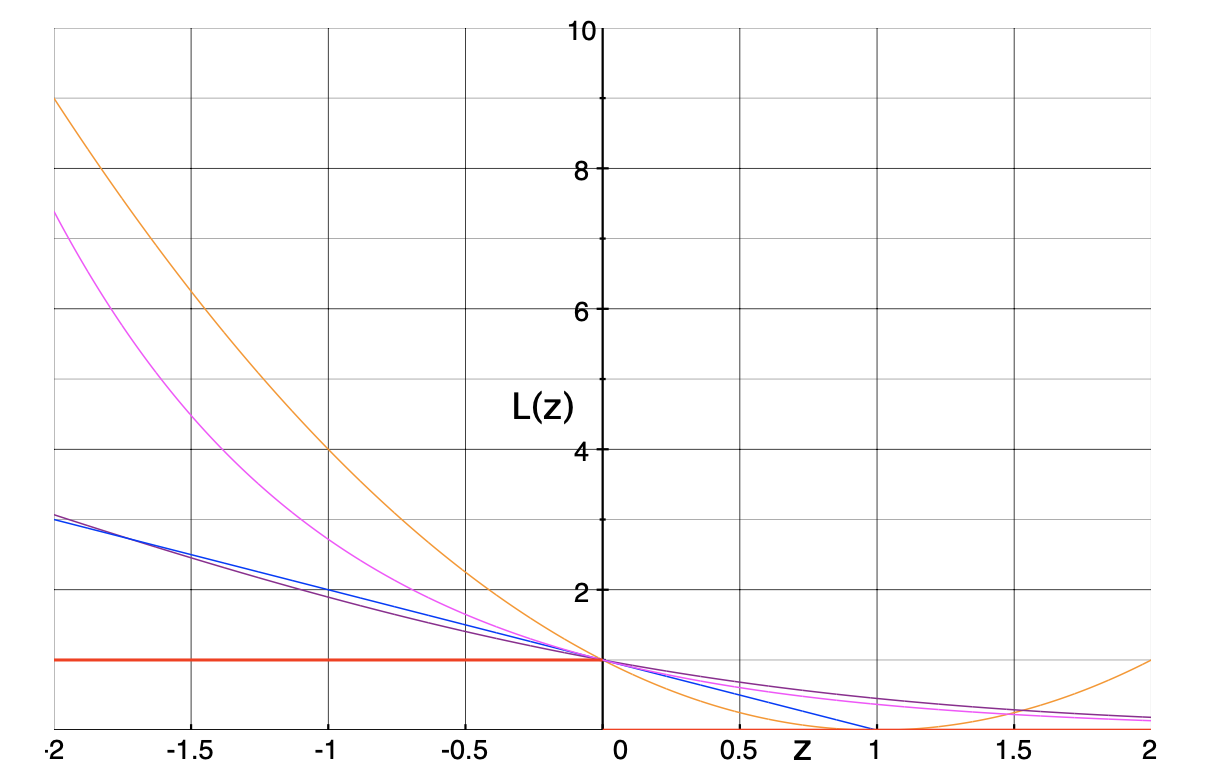
\includegraphics[scale=0.5]{images/allLoss.png}
    \label{fig:enter-label}
\end{figure}

\newpage

\section{Ranking}
Il classificatore rimane binario, ma in output v\textbf{oglio classificare le classi dalla più alla meno probabile}. Ovviamente dopo una scoring function, è facile costriure una ranking function.

Come valutiamo la bontà del ranking? Possiamo usare il \textbf{ranking error rate}, definito come:
\begin{equation}
    rank-err=\frac{\sum_{x\in Te^+,x^{'}\in Te^-}I[\hat{s}(x)<\hat{s}(x^{'})]+\frac{1}{2}I[\hat{S}(x)=\hat{s}(x^{'})]}{Pos\cdot Neg}
\end{equation}
$x$ è l'esempio positivo e $x^{'}$ è quello negativo; se lo score $x$ è più piccolo dello score di $x^{'}$ (quindi sto ordinandoli in modo sbagliato, dovrei mettere prima gli esempi positivi e poi i negativi), \textbf{aggiungo un punto d'errore} allo score che sto calcolando. \textbf{Aggiungo 0.5 punti se gli score dei due esempi sono uguali}; in questo caso non è un errore vero e proprio ma si conta come mezzo punto di errore.

Un \textbf{ranking perfetto} corrisponde ad un numeratore uguale a 0 mentre se un \textbf{ranking completamente sbagliato} è allora la parte che conta gli uguali è 0 ma l'altra è sempre vera (per ogni coppia possibile, quindi per $Pos\cdot Neg$ coppie), quindi il ranking error sarebbe uguale ad 1.

\textbf{Facciamo un esempio:}
\begin{figure}[!h]
    \centering
    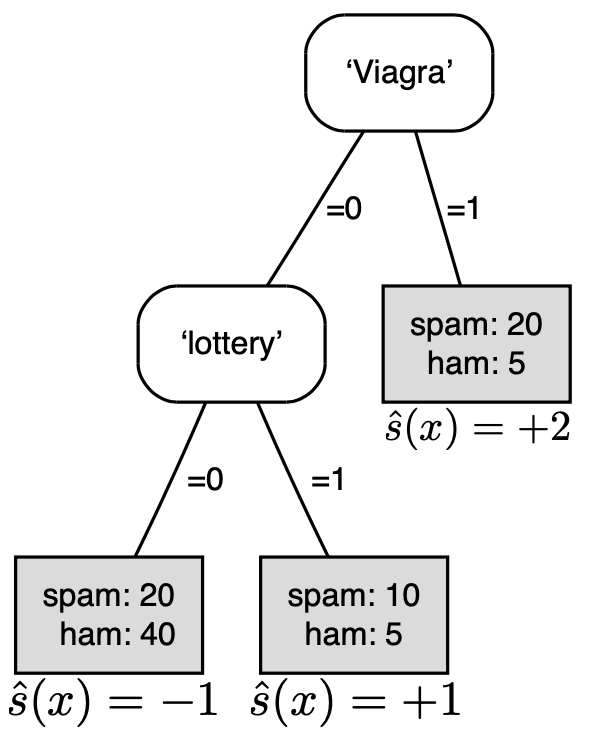
\includegraphics[scale=0.6]{images/rankError.png}
    \label{fig:enter-label}
\end{figure}


Chiameremo:
\begin{itemize}
    \item foglia 1, la foglia che ha spam:20, ham 5;
    \item foglia 2, la foglia che ha spam:20, ham 40;
    \item foglia 3, la foglia che ha spam:10, ham 5;
\end{itemize}
Cominciamo dalla foglia 1, abbiamo che quei 5 esempi negativi (ham) sono classificati in una posizione più alta rispetto ai 20 positivi (spam:20) della foglia 2 e anche rispetto ai 10 (spam:10) della 3. Lo diciamo perchè hanno uno score maggiore. Quindi $5\cdot 10 = 50$ (per la foglia 3), $5\cdot 20 = 100$ (per la foglia 2) $=150$ punti di errore.  

I 5 positivi della foglia 3 sono messi più in alto dei 20 positivi della foglia 2, quindi 100 punti di errore.

Infine calcoliamo i mezzi punti; sono 475 divisi in $20\cdot 5=\frac{100}{2}$ per la foglia 1, $20\cdot 40=\frac{800}{2}$ per la foglia 2 e $10\cdot 5=\frac{50}{2}$ per la foglia 3.

Abbiamo un totale di $475+100+150=725$ errori su 2500 esempi.

\newpage

\section{Stima delle probabilità}
Questo è un caso simile a quello dello scoring ma qui mettiamo un vincolo ulteriore agli score, imponendo che siano tutti posiviti e la loro somma sia 1. In simboli
\begin{equation}
    \hat{p}:X\rightarrow [0,1]^k
\end{equation}
con
\begin{equation}
    \hat{p}(x)(\hat{p_1}(x),\dots,\hat{p_k}(x)).
\end{equation}
Se abbiamo solo due classi, $\hat{p}(x)$ denota la probabilità stimata per la classe positiva.

\paragraph{Probability estimation tree.} Per assegnare le probabilità alle foglie, prendiamo gli esempi che ricadono in quella foglia e diciamo che la probabilità che un esempio capiti in quella foglia è data dal rapporto tra gli esempi cercati e la somma degli esempi ($\frac{20}{20+5}$ per la prima foglia).
\begin{figure}[!h]
    \centering
    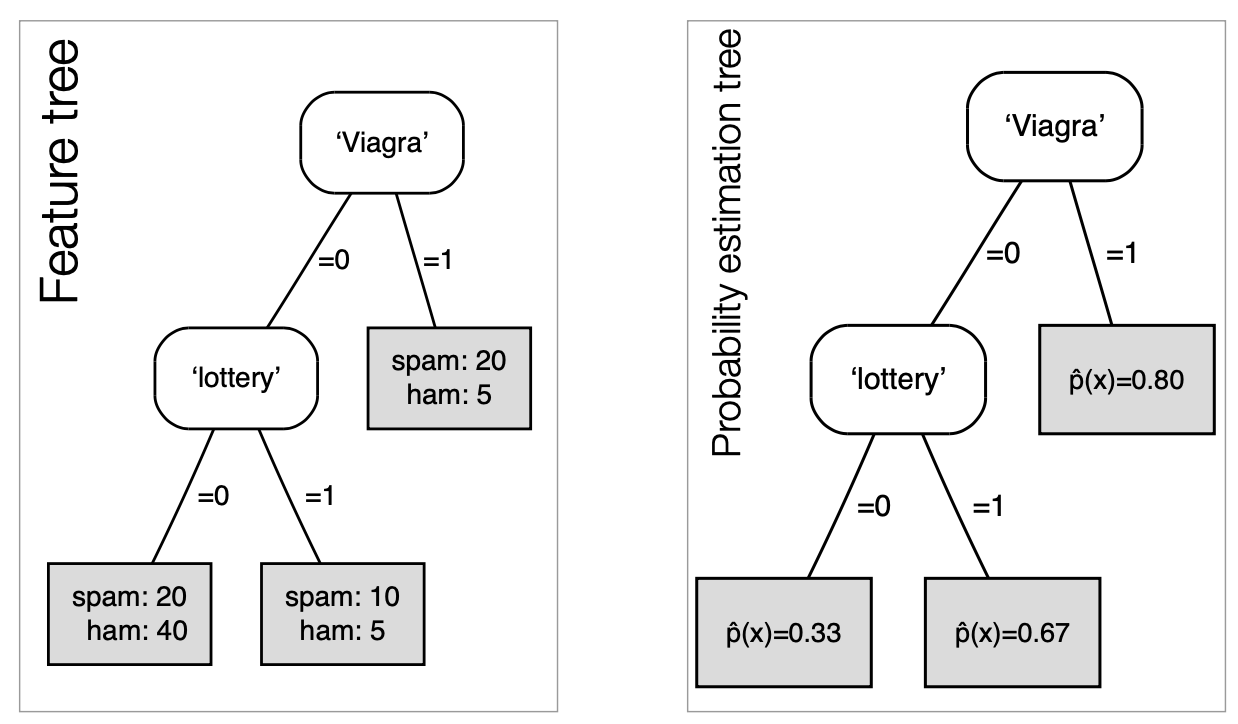
\includegraphics[scale=0.6]{images/probTree.png}
    \label{fig:enter-label}
\end{figure}

Come valuto la bontà delle probabilità emesse? Uso la \textbf{mean squared probability error}, definita così:
\begin{equation}
\begin{split}
    SE(x)=\frac{1}{2}\left|\left| \hat{p}(x)-I_c(x) \right|\right|_2^2 \\
    = \frac{1}{2} \sum_{i=1}^k(\hat{p}_i(x)-I[c(x)=C_i])^2
\end{split}
\end{equation}
dove $I_{c(x)}$ è un vettore che ha 1 nelle posizioni corrispondenti all'etichetta $c(x)$ e 0 nelle altre.

\paragraph{Esempio:}
assumiamo $\hat{p}(x)=(0.7,0.1,0.2)$ e $c(x)=C_1$ e $I_{c(x)}(1,0,0)$.
$SE(x)$ sarebbe valutata come:
\begin{equation}
    \begin{split}
        SE(x)=\frac{\left| \left| (0.7,0.1,0.2)-(1,0,0) \right| \right|_{2}^{2}}{2} \\
        =\frac{\left| \left| (-0.3,0.1,0.2) \right| \right|_{2}^{2}}{2} \\
        =\frac{0.09+0.01+0.04}{2} \\
        =\frac{0.14}{2}=0.07
    \end{split}
\end{equation}

\paragraph{}Quando lavoriamo su un intero dataset facciamo semplicemente la media degli squared error per ogni istanza
\begin{equation}
     MSE(Te)=\frac{1}{\left|Te \right|}\sum_{x\in Te}SE(x)
\end{equation}

\paragraph{Stima delle probabilità empiriche.} Dato un insieme s di esempi etichettati, possiamo stimare la probabilià delle varie classi creando il vettore $\frac{n_i}{S}$ che è il numero degli esempi etichettati con l'etichetta $n_i$ diviso la cardinalità dell'insieme:
\begin{equation}
    \dot{p}(S)=\left(\frac{n_1}{|S|},\dots,\frac{n_k}{|S|}\right)
\end{equation}

\paragraph{Correzione di Laplace.} Se alcune classi sono poco frequenti e abbiamo pochi esempi di esse, è probabile che la stima calcolata poco fa venga 0. Questo è spesso un problema perchè spesso si moltiplicano tutte le probabilità e avere uno 0 rovina tutto. Quindi cerchiamo di fare "smoothing" di queste probabilità, attraverso la correzione di Laplace. L'idea è che assumiamo di aver pescato un esempio in più per ogni classe:
\begin{equation}
    \dot{p}_i(S)=\frac{n_i+1}{|S|+k}
    \label{m-estimate}
\end{equation}

Possiamo anche non applicare uno smoothing uniforme, se in partenza sappiamo che non tutte le classi sono equiprobabili:
\begin{equation}
    \dot{p}_i(S)=\frac{n_i+m\cdot \pi_i}{|S|+m}
\end{equation}
peschiamo $m$ esempi, con $m>k$ e $\pi_i$ probabilità della classe i-esima.

La correzione di Laplace è un caso speciale della (\ref{m-estimate}) con $m=k$ e $\pi_i=\frac{1}{k}$.


\clearemptydoublepage
\chapter{Risultati preliminari}
\section{Dataset}
Nella prima versione sviluppata, il dataset di immagini generate utilizzando PIL è illustrato nelle immagini \ref{fig:out}

\begin{figure}[!h]
  \centering
  \begin{minipage}[b]{0.5\textwidth}
    \tcbox[boxsep=0mm, boxrule=0.5mm, 
            colframe=black!30!black, colback=white]
            {
\includegraphics[width=\textwidth]{pictures/g1.png}}
    % \caption{}
    \label{}
  \end{minipage}
  \begin{minipage}[b]{0.5\textwidth}
    \tcbox[boxsep=0mm, boxrule=0.5mm, 
            colframe=black!30!black, colback=white]
            {
\includegraphics[width=\textwidth]{pictures/g2.png}}
    % \caption{}
    \label{}
  \end{minipage}\\
  \begin{minipage}[b]{0.5\textwidth}
    \tcbox[boxsep=0mm, boxrule=0.5mm, 
            colframe=black!30!black, colback=white]
            {
\includegraphics[width=\textwidth]{pictures/g3.png}}
    % \caption{}
    \label{}
  \end{minipage}
  \begin{minipage}[b]{0.5\textwidth}
    \tcbox[boxsep=0mm, boxrule=0.5mm, 
            colframe=black!30!black, colback=white]
            {
\includegraphics[width=\textwidth]{pictures/g4.png}}
    \caption{In figura sono mostrati 4 esempi di immagini realizzate secondo i criteri illustrati}
    \label{fig:out}
  \end{minipage}
\end{figure}
Le immagini utilizzate come dataset nella prima versione sono semplici immagini 400 x 40 x 1 in cui ho considerato un singolo dominio internet (e.g Google, Facebook, Apple, ...) generando, nel mio caso, 1024 immagini contenenti quel dominio e utilizzando questo set di immagini come Dataset (come input della DCGAN)\\
In una seconda versione ho incluso nelle immagini del dataset, una maschera di rumore per riprodurre un dataset più dinamico e far in modo che il modello generasse caratteri imprecisi (che è proprio il mio scopo). Nella figura \ref{fig:ou2} è possibile notare la densità del rumore (non ho scelto una densità troppo alta, in quanto il modello non risultava convergere).
\begin{figure}[!h]
  \centering
  \begin{minipage}[b]{0.5\textwidth}
    \tcbox[boxsep=0mm, boxrule=0.5mm, 
            colframe=black!30!black, colback=white]
            {
\includegraphics[width=\textwidth]{pictures/a1.png}}
    % \caption{}
    \label{}
  \end{minipage}
  \begin{minipage}[b]{0.5\textwidth}
    \tcbox[boxsep=0mm, boxrule=0.5mm, 
            colframe=black!30!black, colback=white]
            {
\includegraphics[width=\textwidth]{pictures/a2.png}}
    % \caption{}
    \label{}
  \end{minipage}\\
  \begin{minipage}[b]{0.5\textwidth}
    \tcbox[boxsep=0mm, boxrule=0.5mm, 
            colframe=black!30!black, colback=white]
            {
\includegraphics[width=\textwidth]{pictures/a3.png}}
    % \caption{}
    \label{}
  \end{minipage}
  \begin{minipage}[b]{0.5\textwidth}
    \tcbox[boxsep=0mm, boxrule=0.5mm, 
            colframe=black!30!black, colback=white]
            {
\includegraphics[width=\textwidth]{pictures/gg1.png}}
    \caption{La seconda versione del dataset utilizzato dalla DCGAN per produrre immagini. Da notare il rumore aggiunto}
    \label{fig:ou2}
  \end{minipage}
\end{figure}\\
%%%%%%%%%%%%%%%%%%%%%
Una versione più avanzata del modello sarebbe quella di generare immagini aventi padding arbitrario come mostrato in figura \ref{fig:out3}.
\begin{figure}[!h]
  \centering
  \begin{minipage}[b]{0.5\textwidth}
    \tcbox[boxsep=0mm, boxrule=0.5mm, 
            colframe=black!30!black, colback=white]
            {
\includegraphics[width=\textwidth]{pictures/gg1.png}}
    % \caption{}
    \label{}
  \end{minipage}
  \begin{minipage}[b]{0.5\textwidth}
    \tcbox[boxsep=0mm, boxrule=0.5mm, 
            colframe=black!30!black, colback=white]
            {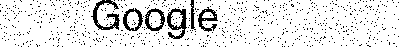
\includegraphics[width=\textwidth]{pictures/gg2.png}}
    % \caption{}
    \label{}
  \end{minipage}\\
  \begin{minipage}[b]{0.5\textwidth}
    \tcbox[boxsep=0mm, boxrule=0.5mm, 
            colframe=black!30!black, colback=white]
            {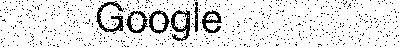
\includegraphics[width=\textwidth]{pictures/gg3.png}}
    % \caption{}
    \label{}
  \end{minipage}
  \begin{minipage}[b]{0.5\textwidth}
    \tcbox[boxsep=0mm, boxrule=0.5mm, 
            colframe=black!30!black, colback=white]
            {
\includegraphics[width=\textwidth]{pictures/gg4.png}}
    \caption{Questa versione del dataset presenta padding randomico su entrambi gli assi.}
    \label{fig:out3}
  \end{minipage}
\end{figure}\\
Infine, un'ultima challenge sarebbe quella di produrre un modello che sia in grado di generare immagini, da un dataset di ingresso che utilizza più font, come quelli mostrati in figura \ref{fig:out4}
\begin{figure}[!h]
  \centering
  \begin{minipage}[b]{0.5\textwidth}
    \tcbox[boxsep=0mm, boxrule=0.5mm, 
            colframe=black!30!black, colback=white]
            {
\includegraphics[width=\textwidth]{pictures/am1.png}}
    % \caption{}
    \label{}
  \end{minipage}
  \begin{minipage}[b]{0.5\textwidth}
    \tcbox[boxsep=0mm, boxrule=0.5mm, 
            colframe=black!30!black, colback=white]
            {
\includegraphics[width=\textwidth]{pictures/am2.png}}
    % \caption{}
    \label{}
  \end{minipage}\\
  \begin{minipage}[b]{0.5\textwidth}
    \tcbox[boxsep=0mm, boxrule=0.5mm, 
            colframe=black!30!black, colback=white]
            {
\includegraphics[width=\textwidth]{pictures/am3.png}}
    % \caption{}
    \label{}
  \end{minipage}
  \begin{minipage}[b]{0.5\textwidth}
    \tcbox[boxsep=0mm, boxrule=0.5mm, 
            colframe=black!30!black, colback=white]
            {
\includegraphics[width=\textwidth]{pictures/am4.png}}
    \caption{Questo dataset presenta immagini con domini scritti utilizzando font differenti.}
    \label{fig:out4}
  \end{minipage}
\end{figure}
\section{Dati generati}
Una volta prodotto il dataset, ho utilizzato la DCGAN per analizzare le immagini che era in grado di produrre, cercando di lavorare sui vari strati convoluzione/deconvoluzione in modo da renderla il più fedele possibile.\\
Dalla prima versione del dataset [\ref{fig:out}], il modello non è riuscito a produrre immagini che rappresentassero in maniera corretta i domini squatted, il problema risiedeva nel fatto che il dataset di partenza era troppo statico (le immagini erano completamente identiche l'une dalle altre). Questo non ha permesso alla rete di produrre immagini con sufficiente rumore tra le singole lettere. In figura \ref{fig:v1} è visualizzato l'output del modello nella versione 1, mentre in figura \ref{fig:lossesv1} un estratto della losses dopo 1000 epoch.
\begin{figure}[!h]
  \centering
  \begin{minipage}[b]{\textwidth}
    
\includegraphics[width=\textwidth]{pictures/picsv1.png}
    \caption{I risultati del modello nella prima versione del dataset}
    \label{fig:v1}
  \end{minipage}
  \hfill
\end{figure}

\begin{figure}[!h]
  \centering
  \begin{minipage}[b]{0.9\textwidth}
    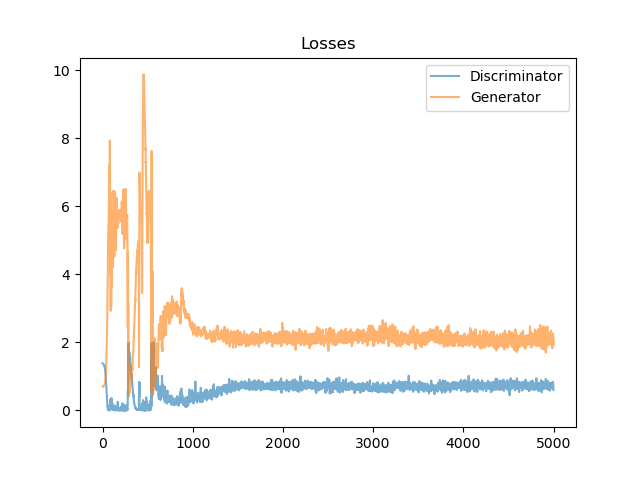
\includegraphics[width=\textwidth]{pictures/lossesV1.png}
    \caption{losses nella versione 1. Da notare che il generatore ha una loss abbastanza alta rispetto al discriminatore}
    \label{fig:lossesv1}
  \end{minipage}
  \hfill
\end{figure}
Nella seconda versione, avendo immagini con rumore casuale all'interno del dataset, la rete converge in maniera più corretta verso le immagini reali producendo anche testo avente lettere distorte dal rumore (che è proprio quello che si vuole produrre). In figura \ref{fig:dcganv2} un esempio di output per la seconda versione del modello. In figura \ref{fig:lossesv2} l'andamento delle losses nell'arco di 1000 epoche.
\begin{figure}[!h]
  \centering
  \begin{minipage}[b]{\textwidth}
    
\includegraphics[width=\textwidth]{pictures/maxpool.png}
    \caption{Output della DCGAN nella seconda versione. Il test è stato effettuato sul dominio "Outlook". Questi sono i risultati dopo 1000 epoche.}
    \label{fig:dcganv2}
  \end{minipage}
  \hfill
\end{figure}

\begin{figure}
  \centering
  \begin{minipage}[b]{0.7\textwidth}
  \tcbox[boxsep=0mm, boxrule=0.4mm, 
            colframe=black!10!black, colback=white]
            {
\includegraphics[width=\textwidth]{pictures/staticv1.png}}
    \label{fig:git1}
  \end{minipage}
  \begin{minipage}[b]{0.7\textwidth}
    \tcbox[boxsep=0mm, boxrule=0.4mm, 
            colframe=black!10!black, colback=white]{
            
\includegraphics[width=\textwidth]{pictures/singlev1.png}}
    \caption{Immagine prodotta dalla DCGAN dopo 1000 epoche rispetto ad un'immagine del dataset di partenza}
    \label{fig:singlev1}
  \end{minipage}
\end{figure}

\begin{figure}[!htb]
  \centering
  \begin{minipage}[b]{\textwidth}
    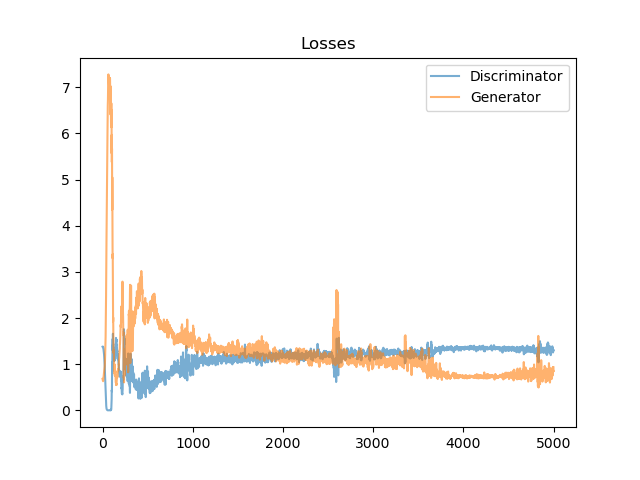
\includegraphics[width=\textwidth]{pictures/loss_maxpool.png}
    \caption{losses utilizzando la seconda versione del dataset. In questa versione la losses è nettamente più decente rispetto alla prima versione.}
    \label{fig:lossesv2}
  \end{minipage}
  \hfill
\end{figure}
Ho anche provato ad usare dei layer di AveragePooling anzichè MaxPooling ma le immagini generate (figura \ref{fig:avgpool}) si presentano molto più sfocate, come previsto.
\begin{figure}[!h]
  \centering
  \begin{minipage}[b]{\textwidth}
    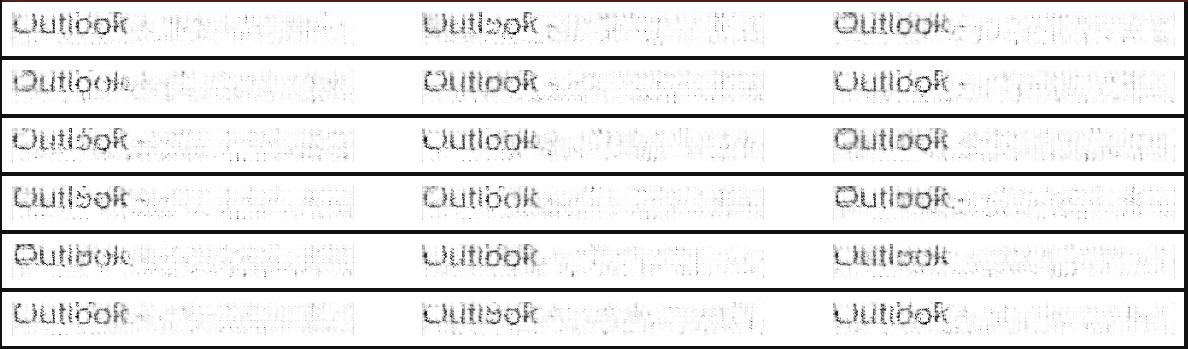
\includegraphics[width=\textwidth]{pictures/avgpool.png}
    \caption{DCGAN nella versione 2. Le immagini generate utilizzando layers di AvgPool al posto di MaxPooling le quali presentano troppe sgranature}
    \label{fig:avgpool}
  \end{minipage}
  \hfill
\end{figure}\\

\section{Validazione}
Utilizzando keras come OCR sono riuscito a produrre delle stringhe di testo partendo dalle immagini in output della rete neurale. Nella prima versione del dataset, non si è riusciti ad estrarre una quantità di domini rilevanti, in quanto le immagini prodotte [\ref{fig:v1}] risultavano appunto prive di rumore e imprecisioni sui caratteri.\\
Per estrarre i potenziali domini di squatting, ho allenato il modello inizialmente con la prima versione del dataset [\ref{fig:v1}] fino a 1000 epoche di addestramento (per le successive versioni del dataset ho utilizzato lo stesso approcio). Successivamente ho fatto produrre alla rete delle immagini di test che ho utilizzato come input per il modulo OCR (Keras). Il modulo OCR produceva una quantità di domini non rilevante e soprattutto con ripetizioni. Ho utilizzato un algorimo per la rimozione dei duplicati ma risultavano essere comunque rilevanti. Il problema non era il fatto che fossero tanti ma che alcuni domini riconosciuti si discostavano troppo da quello che era il dominio di partenza. Per ovviare a questo problema ho utilizzato un algoritmo di Edit Distance (The Levenshtein distance algorithm) per estrarre solo i domini che si discostassero di una certa edit distance dal dominio di partenza. Inzialmente utilizzando come valore di limite 5, ma infine come valore ottimale ho osservato che andasse bene 3.
Qui una lista di potenziali domini di squatting estratti dal Modulo OCR utilizzando la prima versione de dataset.

\begin{verbatim}
outlook,outlock,outlogk,cutlock,outosk,cutgo,cutlook,outlgok,cutlgok,
cutloss,outloock,utogks,wlook,outlouk,outrok.

apple,acoli,pplet,applet,aple,updle,spple,apute,narlle,aprle,appiet,applel,
cpple
\end{verbatim}

Utilizzando invece la seconda versione del dataset, introducendo il rumore alle immagini, si è visto un aumento dei potenziali domini prodotti. Qui una lista per i domini più famosi.

\begin{verbatim}
gutlook,cltlook,cutlook,cutook,dutlook,butlook,butook,gatlook,
cutiook,sutook,sutlook,outlook,sutiook,dutloor,gutook,cutloo,sltlook,
eatlook,eutlook,outiook,duatlook,cutloek,gutloek,cuttook,dutook,suatlook,
outook,dutiook,eutiook,outlooks,autloor,mutlook,suttook,dutlock,oatiook,
oltlook,utook,outtook,sutlock,sutlookk,wutlook,buttook,dutloon,butiook,
cutleok,sutloek,atlook,gutloon,wetlook,gltlook,gutiook,outlooke,outioon,
outloor,cutloor,ontiook,catlook,guatlook,mutook,guttook,putloor,utlook,
cuatlook,gutlock,butlock,oatlook,cutloos,euttook,outlock,sutloor,cutloon,
nutlook,butloak,putloo,duttook,dutloo,bltlook,sutloo,oltook,outloo,dltlook,
butloo,eutlooks,sutloon,eutloor,cutlock,datlook,gutloor,satlook,eutook,
otlook,qutlook,outoek,dutloek,oltlooks,putlook,outlolt,rutlook,olatlook,
dutloos,qutook.

poogle,googe,soogle,google,coogle,gooale,cooge,foogle,saogle,eoogle,gocgle,
oogle,ooge,sooge,cooglle,cooale,cgogle,fooge,gtogle,socgle,goegle,eooge,
ggogle,ooogle,sooale,gdogle,oegle,scogle,sgogle,oocgle,googie,gcogle,saoogle,
sooole,cogle,gogle,fcogle,caoogle,fgogle,fogle,soegle,soosle,sogle,agogle,
googlle,tsoogle.

appias,apdle,saole,faple,appled,adple,sepple,asple,appls,spple,aoples,
eliple,apple,spples,adpls,sltle,appie,apople,aople,atple,acpie,spps,afple,
sapple,fappis,sppie,aple,fapple,applg,faaple,appile,fappie,fadple,ooe,aepie,
applc,aples,aoe,appies,appec,anple,aaple,adplu,sadple,aeals,sadole,adte,
apoles,seple,appe,adols,asol,apples,apole,sadpie,sols,dple,adpole,fapole,
sole,apols,adole,adpe,adpile,acpln,acqie,appla,acole,apile,arple.

amazon,anazon,atazon,aazon,amazan,amnazon,asenazon,aanazon,amezon,
aeazon,eazoc,aaazor,asmazoe,aaazon,aetazon,aazor,armazon,amelzon,amaaon,
amaizon,aeton,ameion,aazos,aaezon,ametzan,amaon,amzon,mazon,amason,
aiazon,amaizan,amtton,amtazon,ameizon,arnazon,amezan,atmazen,ameszon,
rmazon,aanezon,aegazon,aatazon,atazen,amezen,smazon,samazon,aesazon,
aseazon,araen,asmazon,agazon,dazon,amazn,aeaon,orazo,pazon,aezon,amazo,atmazon,
aenazon,anaon,famazon,aazoe,aoazon,anatzon,asnazon,aareon,amaton,auazon,
amazen,anoazon,aazan,ahazon,aaazod,aniizon,aagazos,aeazan,anezon,aagazoen,
ramaizon,amazoe,amaor,annazon,amrzon,
\end{verbatim}



\clearemptydoublepage
\chapter*{Conclusione e lavori futuri}
Il lavoro sviluppato fino ad ora è sicuramente un punto di inizio per creare un sistema completo in grado di produrre in modo proattivo dei domini di squatting di tutte le tipologie elencate ad inizio articolo. In primo luogo bisognerebbe adattare la rete neurale ad essere in grado di auto apprendere il fatto che alcuni tipi di rumori sono utili per l'obbiettivo che vogliamo raggiungere.\\
In secondo luogo è necessario utilizzare un OCR in grado di riconoscere alfabeti differenti in modo da generare domini omografici più complessi che comprendano lettere di alfabeti differenti in quanto i domini generati e riconosciuti dalla versione attuale comprendono solo lettere dell'alfabeto inglese. Utilizzando Keras come OCR, ed essendo anch'esso una rete neurale, ho caricato i pesi necessari al riconoscimenti di lettere dell'alfabeto inglese, bisognerebbe caricare un HDF (Hierarchical Data Format) consono al riconoscimento di altri alfabeti oltre quello inglese.
Per completare il lavoro bisognerebbe aggiungere un modulo supplementare successivo all'OCR in grado di individuare quali, tra i domini riconosciuti e prodotti da SquatGAN, sono effettivamente attivi e potenziali siti di phishing. Questo sarebbe possibile farlo attraverso semplici lookup DNS.
L'architettura spiegata in figura \ref{fig:arch1} risulterebbe quindi come quella mostrata in figura \ref{fig:arch2}
\begin{figure}[!h]
  \centering
  \begin{minipage}[b]{0.6\textwidth}
    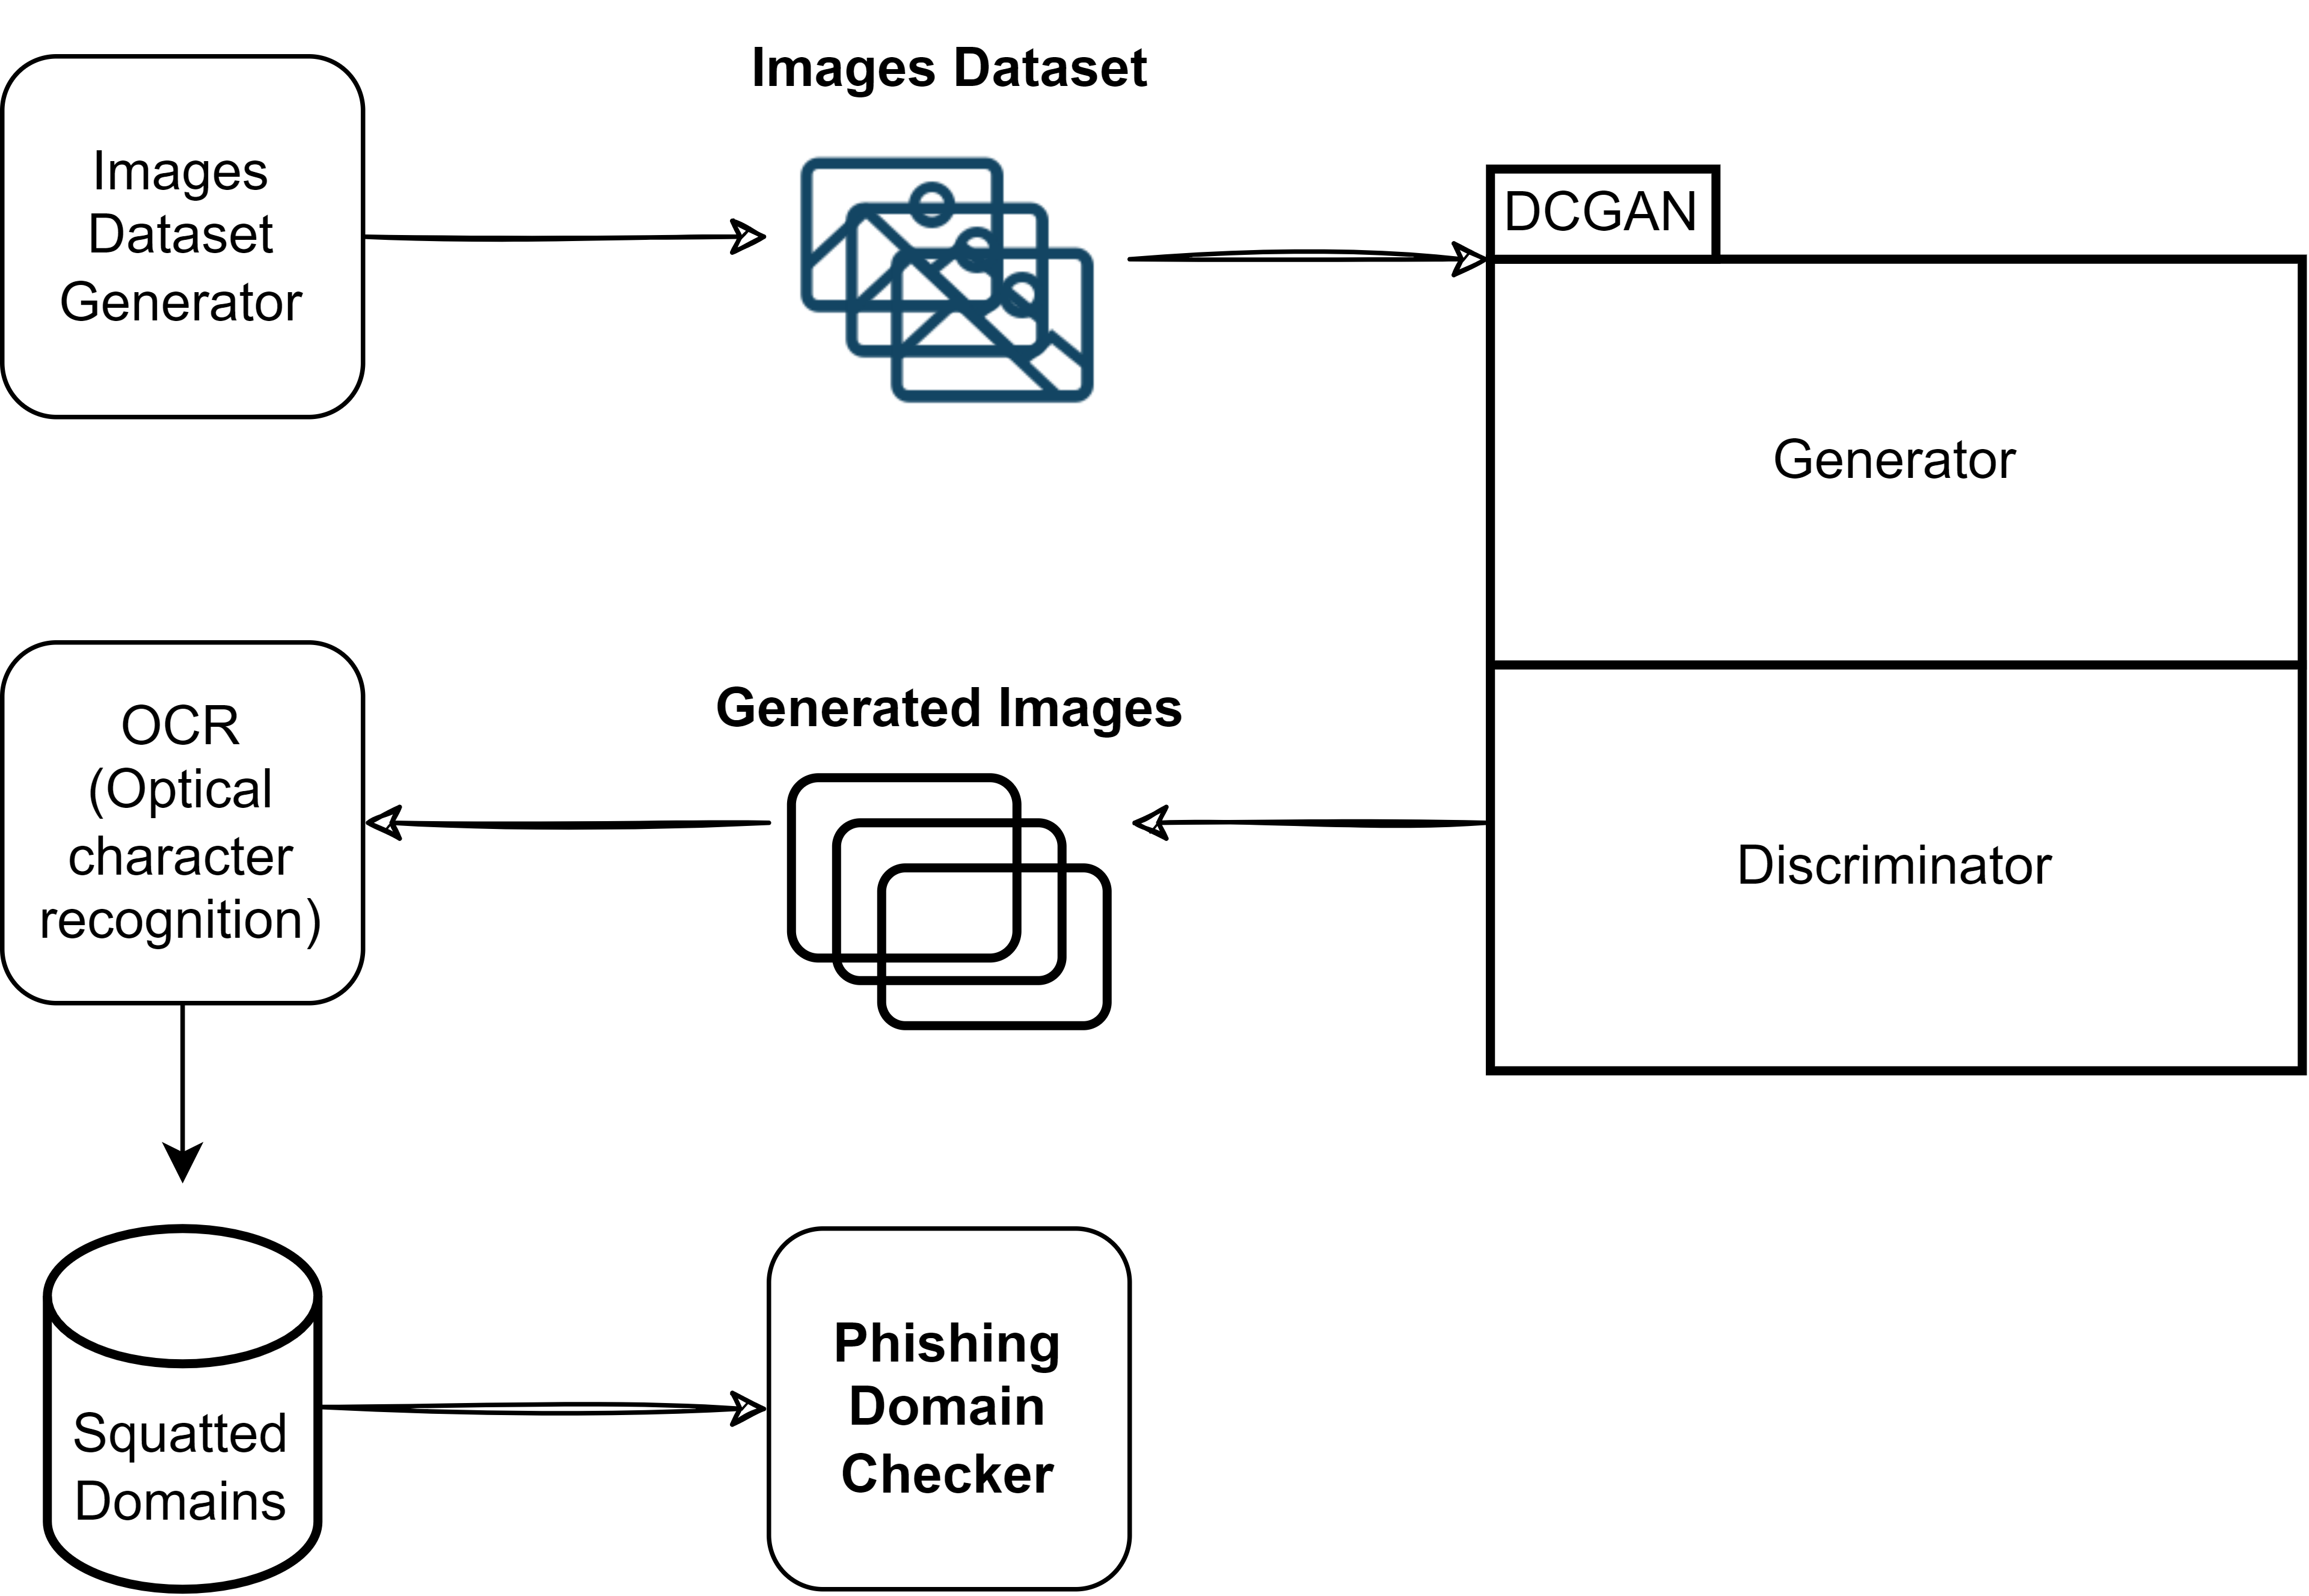
\includegraphics[width=\textwidth]{pictures/arch2.png}
    \caption{un'ipotetica SquatGAN Architecture futura}
    \label{fig:arch2}
  \end{minipage}
  \hfill
\end{figure}\\

\clearemptydoublepage

%%%% TAIL OF THE DOCUMENT
\backmatter
\clearemptydoublepage
%bibliography
\addcontentsline{toc}{chapter}{Bibliografia}
\bibliography{bibliography/bibThesis}
\bibliographystyle{ieeetr}
\clearemptydoublepage


\end{document}
